\chapter{Introduction and Background}

\section{Introduction}

In practical acoustic environments, reflections give rise to reverberation, which is perceived as a sustained decaying tail following the onset of acoustic signals. Reverberation blurs acoustic cues which has a negative impact on speech perception, especially for listeners who are hearing impaired. Even if reverberation is not signficant enough to impact speech intelligibility, it still may have a significant impact on listening effort. As such, it is important for sound reproduction systems such as hearing aids to include techniques for managing reverberation. While many dereverberation algorithms have been proposed, this remains a problem with much room for innovation. Additionally, recent advancements in auditory modeling \citep{bruce2017physiologically} have provided new avenues for analyzing the complex impact of reverberation on speech perception, and thus for evaluating the performance of dereverberation algorithms. The purpose of this thesis is to investigate the behavior of recent perceptually motivated predictors of speech intelligibility and listening effort in the context of reverberation, and to employ these predictors in the evaluation of an existing approach to dereverberation. 

Dereverberation algorithms can be generally categorized as reverberation suppression and reverberation cancellation. Reverberation suppression algorithms aim to estimate/remove the most perceptually impactful components of reverberation, usually by means of a time/frequency gain function or by spectral subtraction. Reverberation cancellation algorithms directly estimate and equalize the transfer function of the acoustic space. Many practical approaches consist of a two-stage algorithm including cancellation and suppression. Most of the effective approaches to reverberation cancellation employ multichannel linear-predictive modeling of the a multi-microphone array. Key algorithms in this area include the delay-and-predict algorithm \citep{triki2006delay}, the linear-predictive multiple-input equalization algorithm \citep[LIME, ][]{delcroix2007precise}, and the weighted prediction error algorithm \citep[WPE, ][]{nakatani2008blind}. The focus of this thesis is on the delay-and-predict algorithm.

In this chapter, a review of room acoustics and the perceptual impacts of reverberation is provided. Additionally the impacts of hearing loss on the perceptual encoding of speech are reviewed, and this is related to perception in reverberation. Lastly, existing predictors of speech intelligibility, which have various degrees of auditory modeling, are discussed. As a slightly separate topic, a review of linear prediction theory is provided, which lays the groundwork for some of the key algorithms in the next chapter.

Chapter 2 provides a review of existing approaches to dereverberation, and the performance and limitations of these algorithms are discussed. Delay-and-predict dereverberation \citep{triki2006delay} is proposed as the focal point for the investigation of multichannel linear-predictive approaches to reverberation cancellation to be conducted in this thesis.

In Chapter 3, the impact of various delay-and-predict algorithm parameters and signal/acoustics variables on dereverberation performance are investigated. The results from this initial evaluation are used to tune the algorithm for the perceptual evaluation in the following chapter.

Chapter 4 begins with a proposed method for evaluating the perceptual impacts of reverberation using objective predictors of speech performance, and this method is analyzed for perceptual validity. A final perceptual evaluation method is then presented which analyzes delay-and-predict dereverberation performance on the basis of speech intelligibility / listening effort, speech quality, and clarity (C50). Five predictors of speech intelligibility are employed: the hearing aid speech perception index \citep[HASPI, ][]{kates2022overview}, the neurogram similarity index method \citep[NSIM, ][]{hines2012speech}, the spectro-temporal modulation index \citep[STMI, ][]{zilany2007predictions} and the short-time objective intelligibility measure \citep[STOI, ][]{taal2010short}. For speech quality, two predictors are used: the hearing aid speech quality index \citep[HASPI, ][]{kates2022overview} and virtual speech quality objective listener \citep[VISQOL, ][]{hines2015visqol}. Using this evaluation method, the perceptual benefit of the delay-and-predict algorithm under realistic/practical reverberant conditions is investigated and discussed.

In Chapter 5 the big picture conclusions from the evaluation in Chapter 4 are provided, and future work is proposed.

\section{Acoustics of Reverberation}

This overview of room acoustics was based on \cite{beranek2012acoustics} and \cite{kuttruff2016room}.

\subsection{Room Acoustics}

When sound is produced in a practical room, it interacts with many physical surfaces such as walls, ceilings, floor and objects, resulting in a wide array of reflections and defraction/refraction effects. Surfaces that are smooth and large relative to the wavelength cause the effective plane wave front to be reflected off in an individual direction (i.e., specular reflection). When surfaces are smaller or highly uneven, sound is reflected in many directions (i.e., scattering) resulting in a spreading of energy (i.e., diffuse reflection). Curved surfaces cause sound to be focused for concave curves, or dispersed for convex curves. When reflections are sparse, they are perceived as distinct echoes, while dense concentrations of reflections are perceived as persistance of the direct sound (i.e., reverberation). 

Reflected sound results in a series of wavefronts reaching the listener with different amplitudes and phases, which can be modeled by the convolution of the dry (i.e., clean) speech signal with a sequence of impulses called the room impulse response (RIR). Similarly, the transfer function corresponding to the RIR (i.e., its Z-Transform) is referred to as the room transfer function (RTF). Like any impulse response, the RIR can be convolved with a theoretical source signal to compute the (noise-free) soundfield that would be perceived at a listening location. The sound that arrives at the listener via line-of-sight is called the direct sound, which is typically the first impulse in the RIR.

Symmetric acoustic spaces such as rectangular rooms tend to produce consistent reflection patterns which results in concentration of reflections from particular directions and patterns of constructive and destructive interference throughout the room (i.e., room modes). Irregular room shapes, and the presence of objects in the room result in more scattering of waves, resulting in a sound field that is more symmetric in the dispersion of energy (i.e., more diffuse). In the extreme case, when the direct sound is the same level as the reflections, a diffuse sound field is produced. Under this condition, sound appears to arrive from all directions equally, sound pressure is distributed evenly throughout the room, and phase relationships between waves can be considered uncorrelated.

Reflection is not uniform over frequency, so reflected sound waves have different spectra from their corresponding incident waves. Common surfaces such as walls and fabric tend to have a lowpass response. This effect is particularly pronounced in the presence of multiple reflections, giving typical room frequency responses some roll-off at high frequencies. Room frequency response can be divided into three primary regions: a low frequency ``mode-dominated" region, a mid frequency ``transition" region, and a high frequency ``diffuse field dominated" region. At low frequencies, where wavelengths are similar to room dimensions, standing waves give rise to strong room modes (i.e., room resonances), which results in a frequency response with a smoother pattern of spectral peaks and notches. As frequency increases through the transition zone, these spectral peaks and notches become more dense. Above a frequency threshold called the Shroeder Frequency \citep{schroeder1962frequency}, the reverberant sound field is highly diffuse and the frequency response becomes highly irregular.

\subsection{Early and Late Reflections} \label{section:early_late_reverb}

RIRs are often divided conceptually into three temporal sections: direct sound, early reflections and late reflections (Figure \ref{fig:RIR_EDC_RTF_Example}). The direct sound is an acoustically attenuated version of the transmitted sound, delayed by the time of flight between the sound source and the listening location.  Early reflections are generally considered to be the reflections which arrive within 50 -- 100 \unit{\milli\second} of the direct sound, and late reflections represent the rest of the reflections that follow.  Early reflections are generally not perceived as distinct reflections, instead being integrated with the direct sound by perceptual adaptations which will be discussed later. This results in a perceptual SNR boost of up to of up to approximately \qty{9}{\decibel}, which aids in speech perception. Conversely, late reflections are perceived as distinct from the direct sound and collectively create a dense decaying sound ``tail” after the perceived direct and early sound. This produces the characteristic decaying sustained sound of reverberation (i.e., the reverberant tail), which has a negative impact on speech perception. As such, in the design of an acoustic space for speech perception, the goal is not to minimize reverberation, but rather it is often to minimize late reflections and maximize early reflections. It should be noted however, that for in certain acoustic spaces (e.g., music performance halls), some late reflections are also subjectively preferable. 

\begin{figure}[H]
	\centering
	\begin{subfigure}[b]{0.7\textwidth}
		\centering
		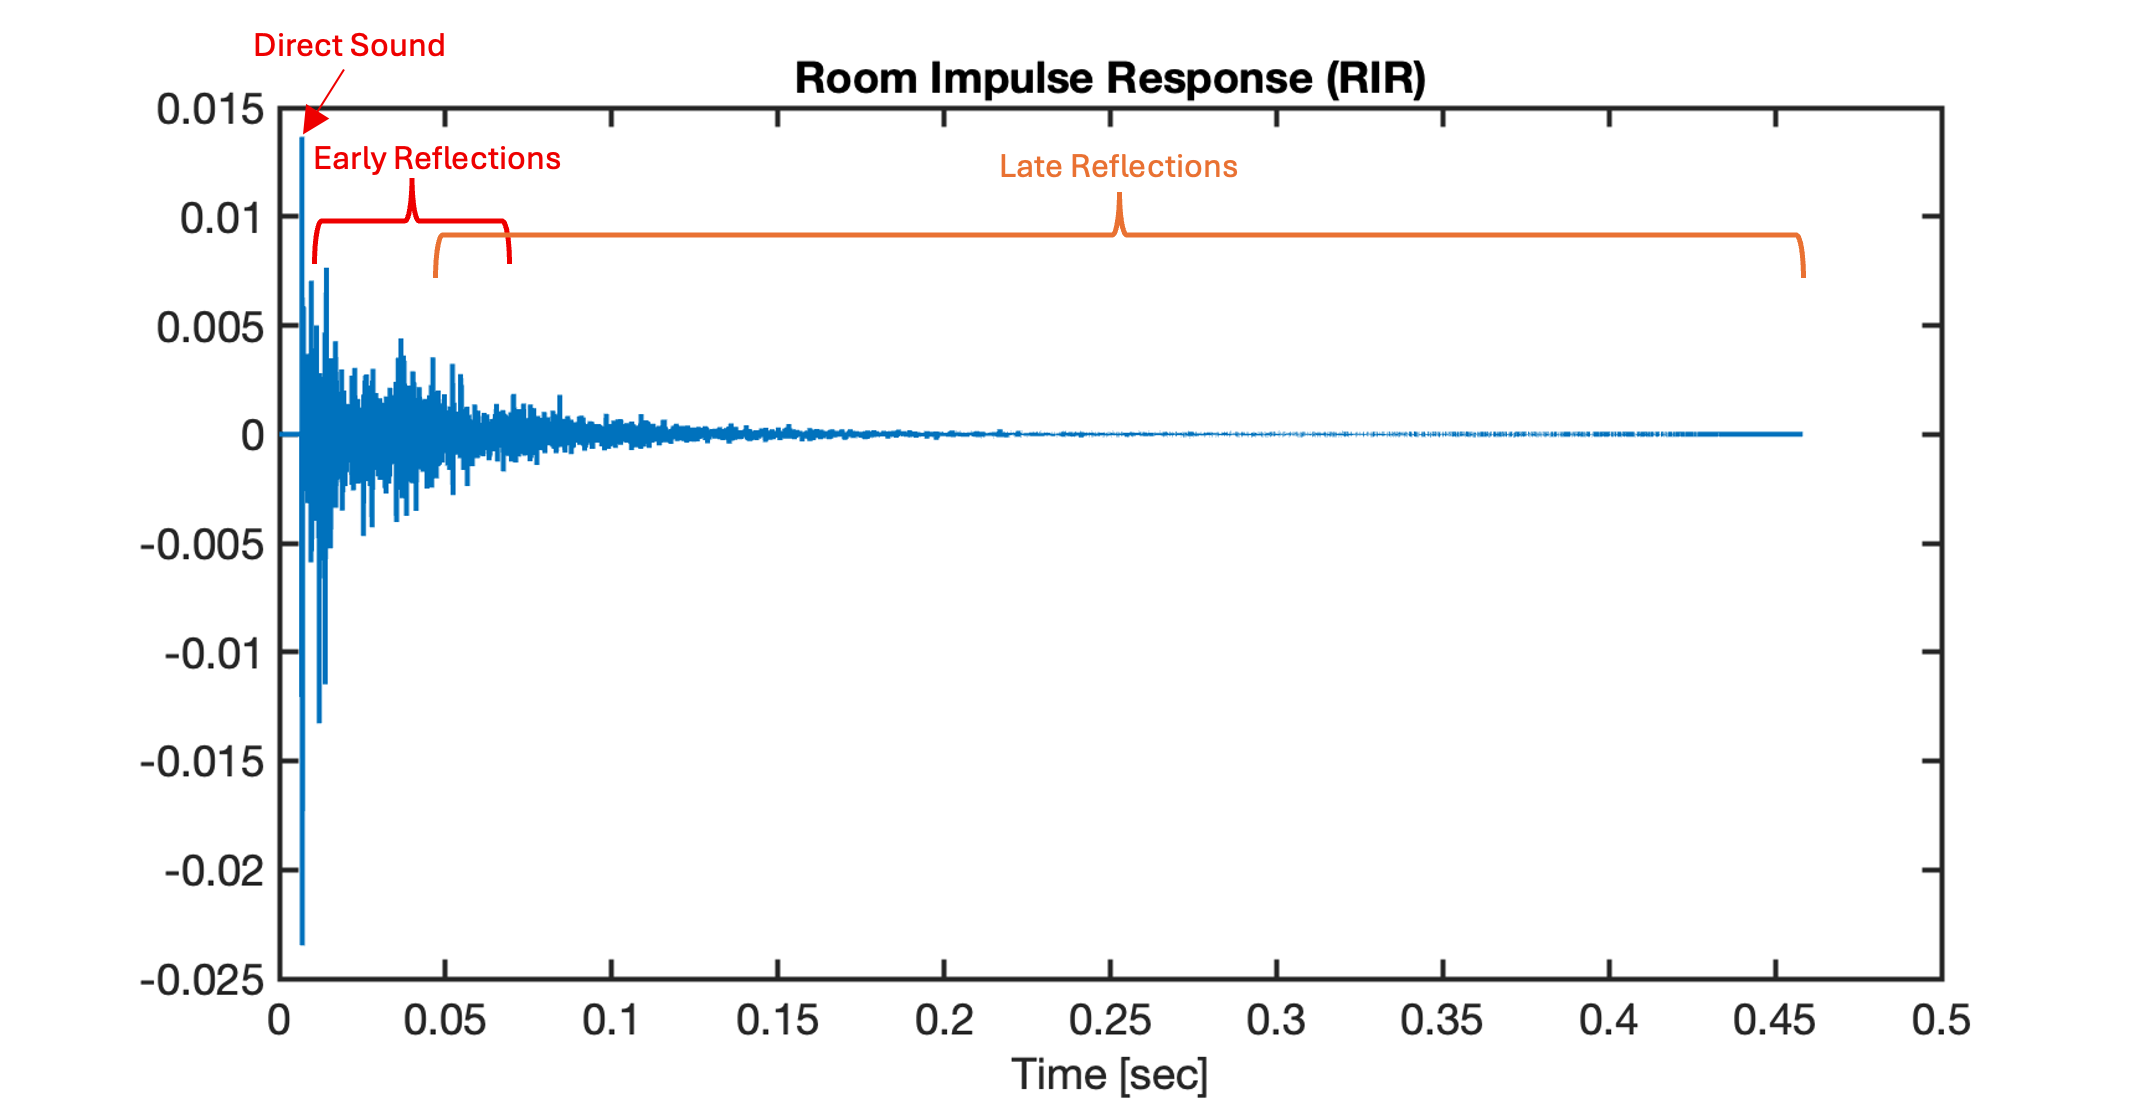
\includegraphics[width=\textwidth]{rir_example_office}
	\end{subfigure}
	\hfill
	\begin{subfigure}[b]{0.7\textwidth}
		\centering
		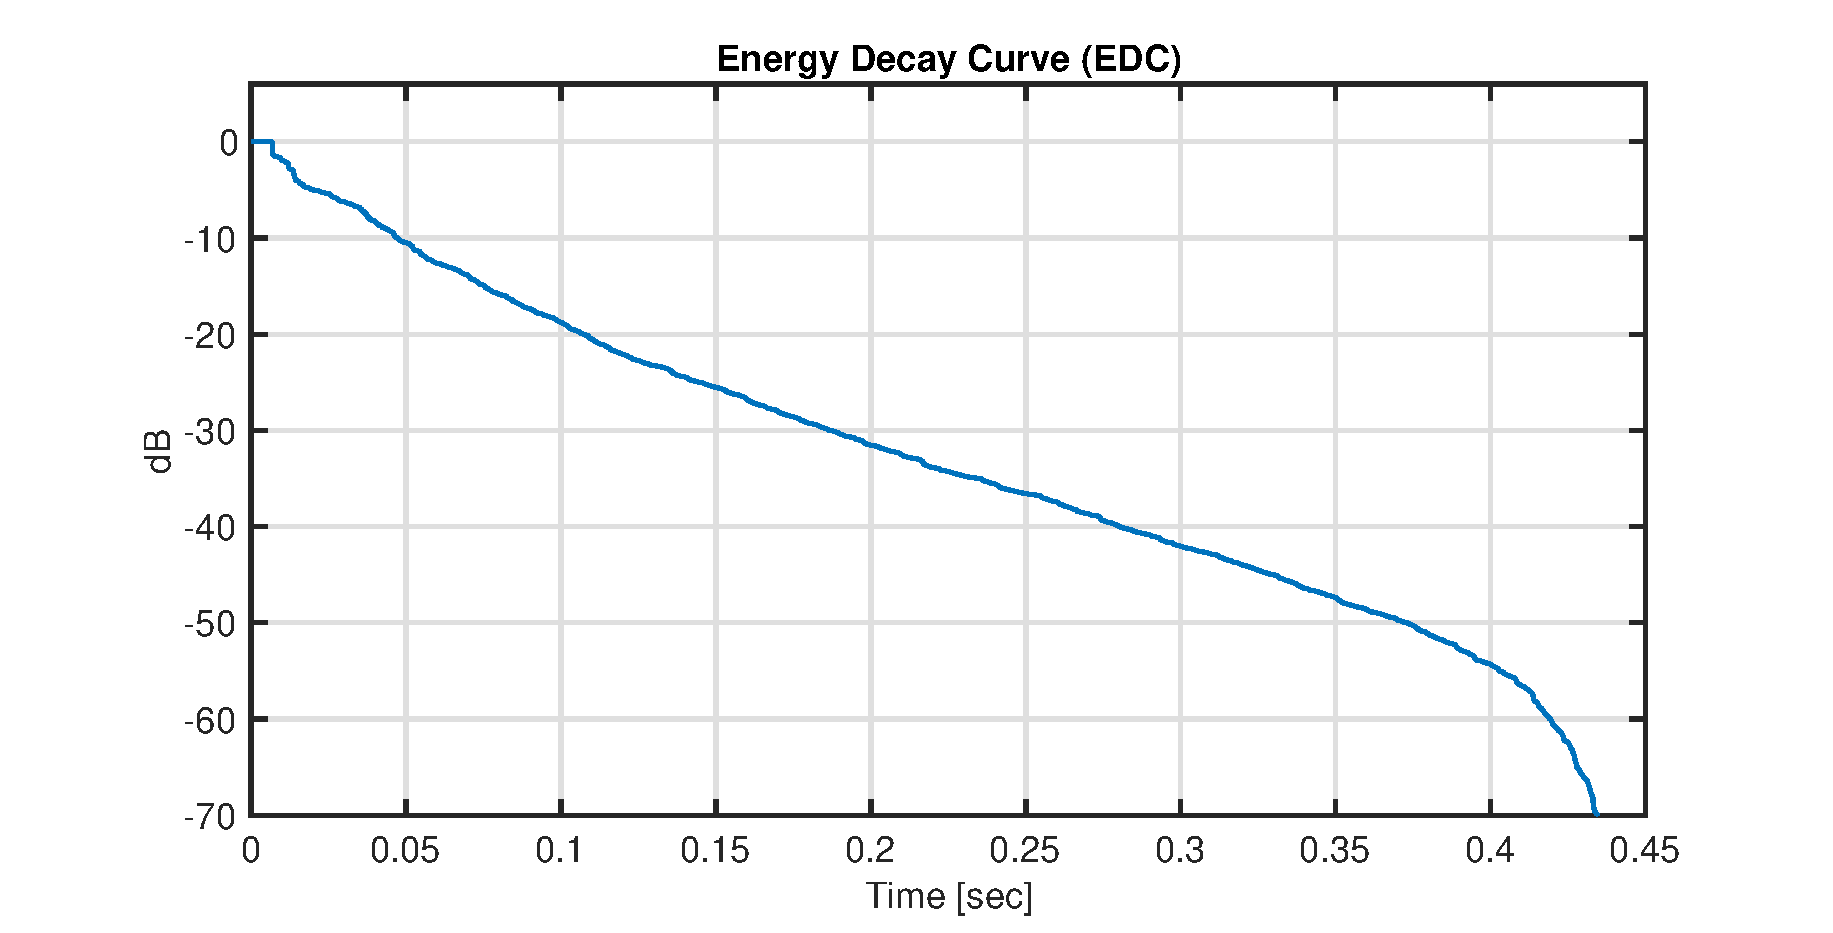
\includegraphics[width=\textwidth]{edc_example_office}
	\end{subfigure}
	\hfill
	\begin{subfigure}[b]{0.7\textwidth}
		\centering
		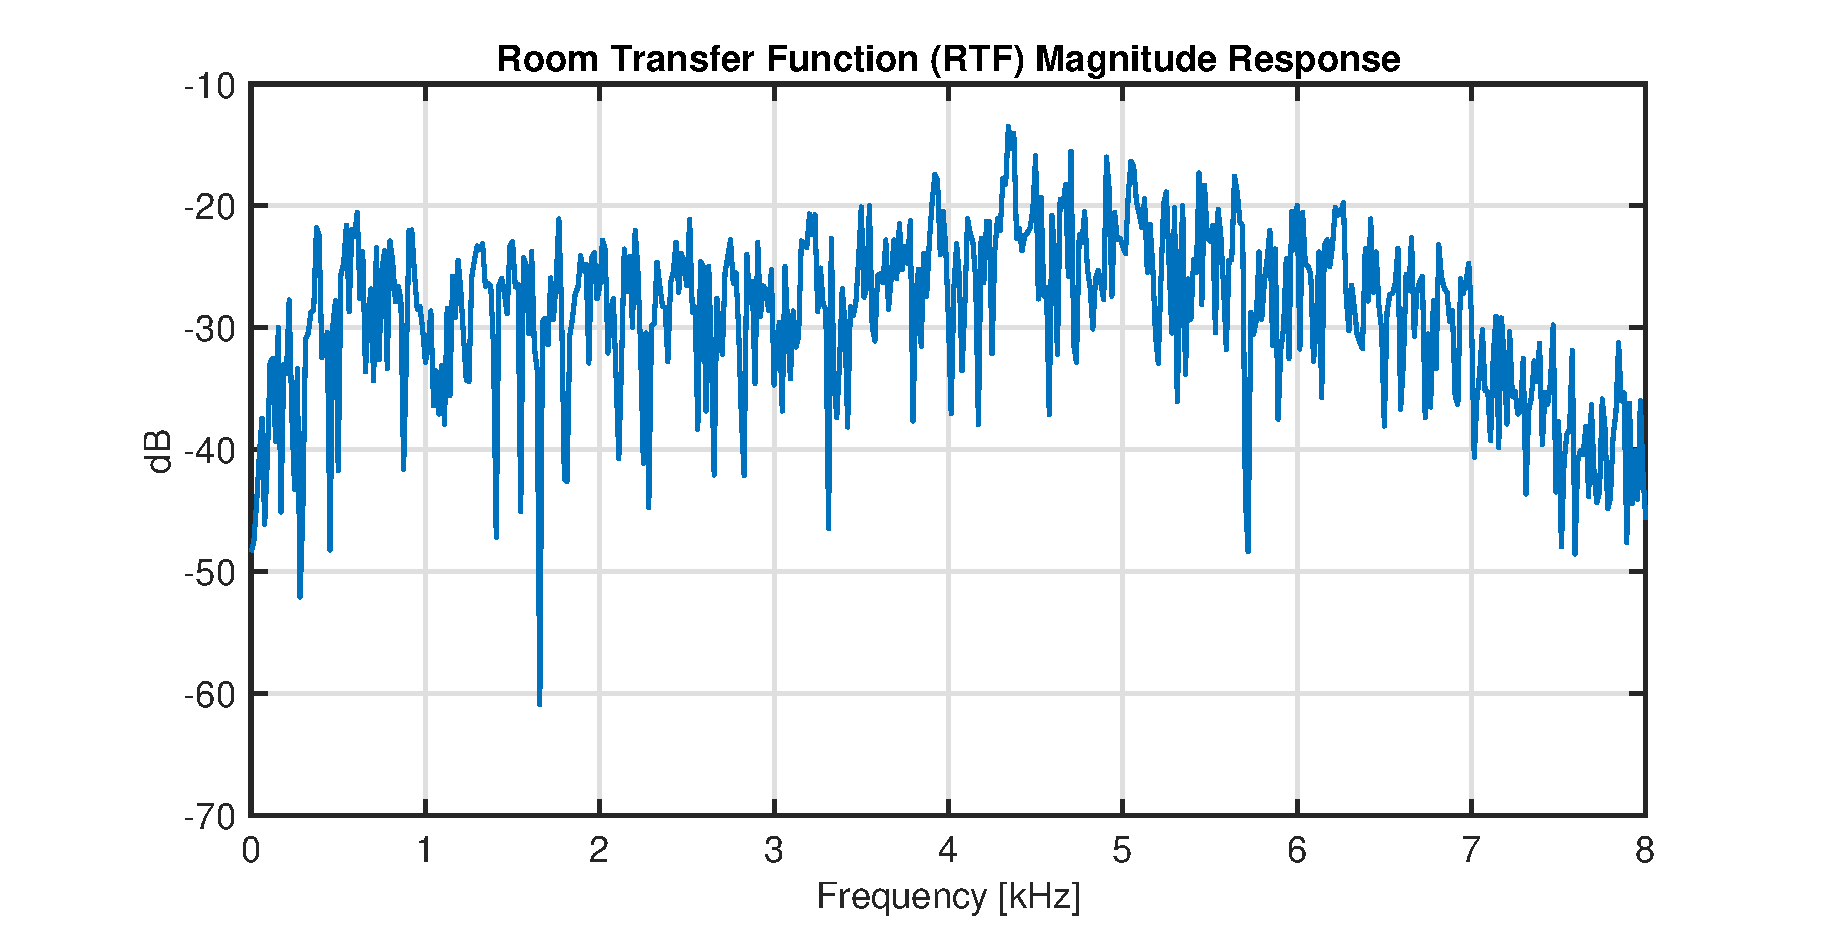
\includegraphics[width=\textwidth]{rtf_example_office}
	\end{subfigure}
	\caption[Example of a room impulse response (RIR), energy decay curve (EDC) and room transfer function (RTF) magnitude response]{Example RIR, EDC and RTF Magnitude Response. RIR is the ``office II" room from the HRIR database \citep{kayser2009database}.}
	\label{fig:RIR_EDC_RTF_Example}
\end{figure}

In simple room geometries and diffuse field conditions, the sound pressure level of reverberation decays exponentially.This is evident in Figure \ref{fig:RIR_EDC_RTF_Example} where the EDC shows approximately linear decay of energy on a logarithmic scale. Early reflections primarily consist of the first reflections off the walls, floor and ceiling of the room. These reflections are more sparse in nature, making the early part of the RIR sporadic and non-exponential. Since late reflections involve many wavefronts produced by repeated reflections around the room, they are much more dense and diffuse in nature. The initial time delay gap (ITDG) between the direct sound and the first early reflection, as well as the duration of these first reflections increases with room size. Although early reflections are not perceptually distinct, they still provide a perceptual sense of room size.

The perceptual distinction between early and late reflections has led to a number of useful metrics which describe amount of reverberation in terms of their relative energies. The direct-to-reverberant ratio (DRR) which is the ratio of direct sound to all reverberant energy expressed in $\unit{\decibel}$, i.e.,

\begin{equation}
	\mathrm{DRR} = 10\log_{10}\left(\frac{\int_{t_d-t_0}^{t_d+t_0}h^2(t)dt}{\int_{t_d+t_0}^{\infty}h^2(t)dt}\right)\;\;\unit{\decibel}
\end{equation}

\noindent
where $h(t)$ is the RIR, $t_d$ is the time of the direct sound, and $t_0$ represents a small window around the direct sound. Typically $t_0$ is approximately $1.0$ to \qty{2.5}{\milli\second}, not the early reflection window. A more perceptually relevant metric is ``clarity" ($C_{t_e}$, commonly $C50$) which is the ratio of direct and early energy to late energy expressed in $\unit{\decibel}$, i.e.,

\begin{equation}
	C_{t_e} = 10\log_{10}\left(\frac{\int_{t_d}^{t_d+t_e}h^2(t)dt}{\int_{t_d+t_e}^{\infty}h^2(t)dt}\right)\;\;\unit{\decibel}
\end{equation}

\noindent
where $t_d$ is the time of the direct sound, and $t_e$ is the duration after the direct sound defined as early reflections (i.e., around \qty{50}{\milli\second} for speech). Another related metric is ``definition" ($D_{t_e}$, commonly $D50$) which is the ratio of direct and early energy to total RIR energy, i.e.,

\footnote{To avoid confusion between clarity/definition implying the metrics of reverberation and the general usage of those words, these metrics will only ever be referred to as $C50$ and $D50$.}

\begin{equation}
	D_{t_e} = 10\log_{10}\left(\frac{\int_{t_d}^{t_d+t_e}h^2(t)dt}{\int_{0}^{\infty}h^2(t)dt}\right)\;\;\unit{\decibel}
\end{equation}

Another common way of analyzing reverberation is using the energy decay curve (EDC), which is a metric of the amount of energy remaining in the RIR $h(n)$ at time $t$.

\begin{equation}
	\mathrm{EDC}(t)=\int_{t}^{\infty}h^2(\tau)d\tau \label{eq:edc}
\end{equation}

Note in Figure \ref{fig:RIR_EDC_RTF_Example} how the EDC decays approximately linearly in the log domain (i.e., exponentially in the linear domain) during late reflections, but is more step-like during early reflections.  The rapid drop off of energy towards the end of the RIR in this example is due to a time window applied during the measurement process \citep{kayser2009database}. The EDC is much smoother than the RIR, making it much more useful for analyzing the decay rate of reverberation.

An extention of the EDC is the energy decay relief (EDR), which uses the short-time fourier transform (STFT) to represent the EDC per frequency band.

\begin{equation}
	\mathrm{EDR}(t_n,f_k)=\sum_{m=n}^{M}|H(m,k)|^2
\end{equation}

\noindent
where $H(m,n)$ is the STFT at time window $m$ and frequency bin $k$, and $M$ is the total number of time windows in the RIR. $t_n$ and $f_k$ represent the equivalent physical times and frequencies.

The most common objective metric of reverberation is reverberation time (RT60, or simply T60) which describes the time required for the reverberant energy to decay by 60 dB, becoming effectively inaudibile. \cite{sabine1922collected} proposed a closed-form estimate for T60 from the volume $V$ in \unit{\metre\cubed} of the room, the surface area $S$ in \unit{\metre\squared} of the room boundary surfaces and the average absorption $\alpha$ of the surfaces.

\begin{equation}
	\mathrm{T}_{60}=\frac{0.161V}{S\alpha}\;\unit{\second}
\end{equation}

Alternatives to T60 are T30 and T20, both of which attempt to estimate T60 from the more exponentially decaying parts of the RIR. T30 performs linear extrapolation of the log-domain EDC from -5 \unit{\decibel} to -35 \unit{\decibel} down to -60 \unit{\decibel}. i.e., T30 is an estimate of T60 based on the first 30 \unit{\decibel} of the EDC. Similarly, T20 estimates T60 based on the first 20 \unit{\decibel} of the EDC. 

Reverberation time alone, however, provides a limited description of reverberant decay, since it is primarily focuses on describing the exponential decay of late reverberant tail and does not give much information about the early portion of the RIR which generally follows a different decay rate. Since two RIRs with the same T60 may have different proportions of early and late reflections, the perceptual impact of those RIRs may be substantially different. As such, the early decay time (EDT) has been introduced to model the early part of the RIR. EDT is a measure of how long the EDC takes to decay by \qty{10}{\decibel}. It is important to note, however, that this early decay region of the the RIR is not necessarily the same as the early reflections. EDT is defined based on a certain amount of attenuation (\qty{10}{\decibel}), whereas early reflections are defined based on a certain time window (around \qty{50}{\milli\sec}). This is an important distinction because, as will be discussed further, the early reflections generally provide a perceptual benefit, while a lower EDT (i.e., a stronger early decay region) may have a negative impact on perception if the early decay region is longer than the boundary between early/late reflections. In this thesis, the two regions of the RIR (described by EDT and reverberation time respectively) will be referred to as the ``early decay region" and ``late decay region".

%\subsection{Numerical Properties of Room Impulse Reponses}

%* Typically non-minimum phase (Not all poles/zeros in U.C.), making them non-invertible (no causal stable inverse exists)
%* May have many perfect zeros (leading to completely unrecoverable content) or near-perfect/strong zeros (leading to effectively unrecoverable content in the presence of noise -- severe noise amplification)
%* Very long (multiple seconds, 1000s of samples)


\section{The Auditory System}

The human auditory system is a complex biological system which has evolved to optimally transform acoustical stimulus into neurological excitations that can be understood by the brain and interpreted as sound. It is made up of many acoustical, mechanical, fluid dynamic, chemical and neurological subsystems, each of which plays a key role in this process.

A detailed description of the auditory system can be found in \cite{pickles2013}, but the important details have been reviewed in this section.

\subsection{The Outer and Middle Ear}

\begin{figure}[H]
	\centering
	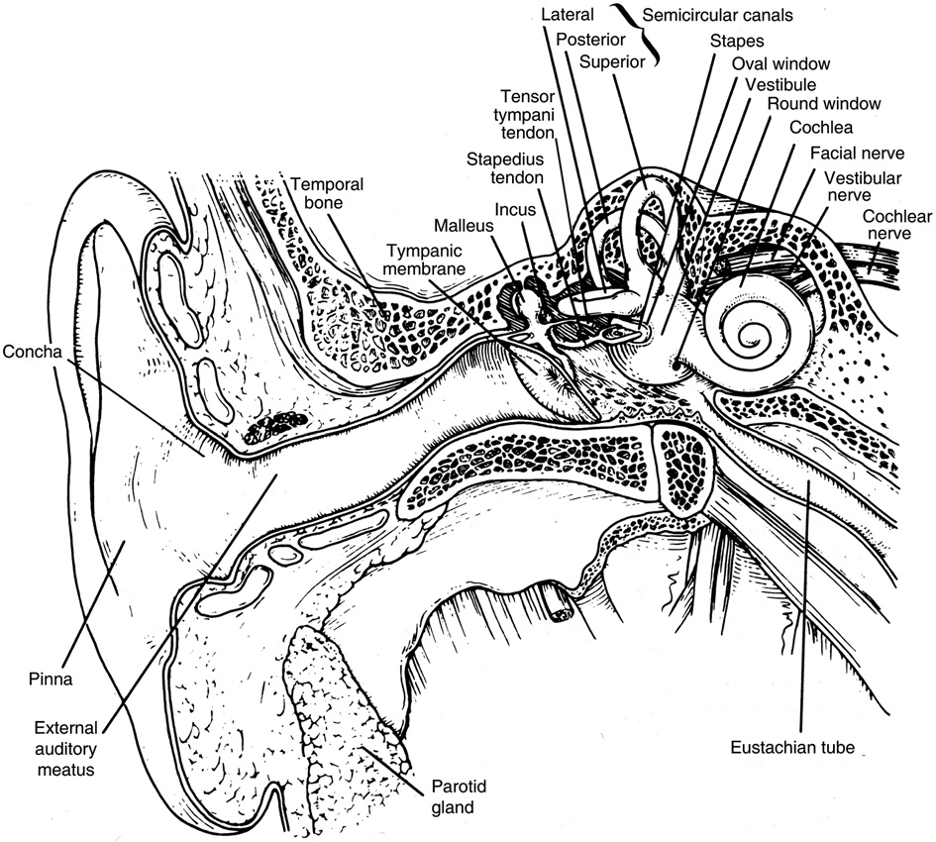
\includegraphics[width=0.65\textwidth]{auditory_system_outer}
	\caption[The human auditory system]{The human auditory system. \textbf{from pickles, no permission yet}}
	\label{fig:auditory_system_outer}
\end{figure}

The outer ear is an acoustical/mechanical system which transfroms and transfers acoustical signals to the middle ear. When air is pushed and pulled by a sound source (e.g., a loudspeaker or glottal pulsing in human speech production), this gives rise to a pattern of compression and rarefraction in the volume of air particles, which propagates away from the sound source as a pressure wave (i.e., an acoustical signal). Acoustical signals in the vicinity of the human ear are collected by the pinna which consists of an exposed cartelage structure (i.e., the flange) and a resonant cavity (i.e., the concha). The sound propagates through the external auditory meatus (i.e., the ear canal) and excites the tympanic membrane (i.e., the ear drum). The shape of the pinna and ear canal maximize transfer of acoustical energy to the ear drum. Additionally, the complex shape of the flange gives rise to a frequency-selective directional response known as a head-related tranfer function (HRTF), which plays an important role in sound localization.

The middle ear transfers the mechanical energy from the vibration of the tympanic membrane to the inner ear via a collection of bones called the ossicles. The three osiccles are the malleus, incus and stapes, and together their rotation/motion performs a lever-like action which trasfers energy from the tympanic membrane to a much smaller flexible membrane-covered opening into the cochlea of the inner ear known as the oval window. The middle ear ossicles act as an impedance-matching mechanical transformer, maximizing energy transfer from the outer ear to the cochlea and minimizing the reflection of energy back into the outer ear.

\subsection{The Inner Ear}

The inner ear consists of two complex fluid-filled bone structures: the vestibular system which is responsible for balance and the cochlea which is responsible for hearing. The cochlea is a spiral-shaped structure made up of three separate bone cavities (i.e., scalae) which extend its full length: the scala vestibuli, scala tympani and scala media. The scala vestibuli and scala tympani share the same cochlear fluid (perilymph) and are connected at the apex of the cochlea by a narrow opening called the helicotrema. The scala media sits between the other two scalae and is filled with a separate cochlear fluid called endolymph. The scala media is separated from the scala tympani by the basilar membrane. 

Inside the scala media, the organ of corti sits on top of the basilar membrane, and is the primary organ involved in transduction of auditory signals. Its base holds thousands of hair cells, each of which have clusters of hair-like structures called stereocilia. The stereocilia connect hair cells on the base of the organ of corti to the upper part of its structure which is called the tectorial membrane. The hair cells are innervated by auditory nerve fibres (ANFs) which carry messages to and from the brain. Inner hair cells (IHCs) are primarily innervated by afferent ANFs which carry auditory sensory information to the brain, whereas outer hair cells (OHCs) are mostly innervated by efferent ANFs which modulate the OHCs' mechanism for active amplification (discussed later).

\begin{figure}[H]
	\centering
	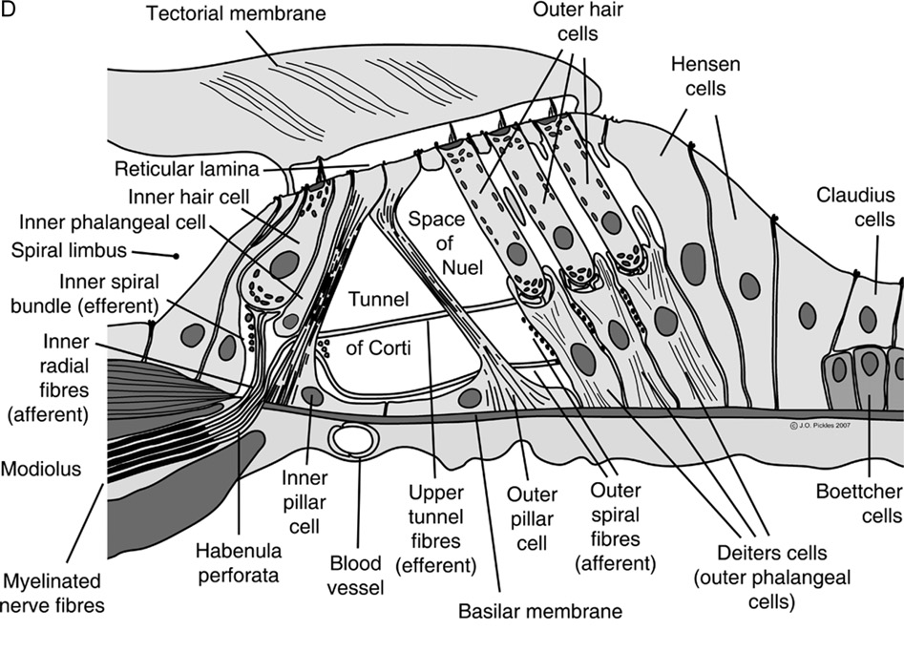
\includegraphics[width=0.65\textwidth]{auditory_system_inner}
	\caption[Cross-section of the organ of corti]{Cross-section of the organ of corti, the primary transduction mechanism of the cochlea. \textbf{from pickles, no permission yet}}
	\label{fig:auditory_system_inner}
\end{figure}

When the middle ear ossicles push the oval window in response to an acoustic stimulus, a pressure wave is induced inside the cochlear fluids. The pressure wave propagates from the oval window at the base of the cochlea, through the scala vistibuli to the apex of the cochlea, and then returns to the base via the scala tympani, reaching the round window. The basilar membrane moves in response to the pressure wave, which in turn moves the organ of corti. The base of the organ of corti moves relative to the more rigid tectorial membrane, causing the stereocilia to flex. This results in the opening/closing of transduction channels which modulate the flow of positively charged ions from the cochlear fluid in the scala media into the hair cells. This modulation to the electrical potential in the hair cells induces an electrical signal into the ANFs via neurotransmitter release.

To summarize, acoustic stimulus propagates through the pinna and ear canal, vibrating the ear drum. The signal is transfered from the ear drum to the oval window of the cochlea by the ossicles in the middle ear. A fluid pressure wave is generated in the cochlear fluids which flexes the stereocilia, modulating current flow into the hair cells and generating an electrical signal in the auditory nerve. 

The electrical signal generated in the ANFs consists of a sequence of spikes. These impulses represent depolarization (i.e., rising phase) and subsequent repolarization (i.e., falling phase) of a neuron cell membrane due to opening and closing of voltage-gated ion channels in the membrane. In the absense of auditory stimulation, action potentials firing continues at a rate called the spontaneous firing rate. Spontaneous firing rates vary from near-zero up to around 160 spikes/sec. At the onset of auditory stimulation, the firing rate increases by approximately 5 -- 30 spikes/sec above the spontaneous rate if the intensity of auditory stimulation is above a certain treshold. Auditory stimuli below this threshold will not produce any detectable change to electrical activity in the auditory nerve, and therefore will not be detected by the brain. This threshold therefore results in a minimum acoustic level that can be detected by the auditory system (i.e., the threshold of hearing). In response to a low frequency sinusoidal stimulus, ANFs do not spike on every cycle of the sinusoid, but when they do always fire at the same phase of the cycle (i.e., ANF firing is phase-locked to the simulus). This phase-locking is key to the perceptual encoding of temporal signal information. For frequencies above approximately 4 -- 5 \unit{\kilo\hertz} this behaviour starts to diminish, which reduces temporal resolution. However, at higher frequencies ANFs tend to be phase-locked to the slower temporal amplitude modulation.

%during exchange of neurotransmitter accross the inter-neuron gap (i.e., the synapse)

\subsection{Tuning, Non-Linearities and Active Amplification in the Cochlea} \label{section:hearing_non_linearities}

At the base of the cochlea, the basilar membrane is narrow and rigid making it sensitive to high frequencies. The basilar membrane becomes progressively wider and less rigid towards the apex, making it more sensitive to low frequencies. This frequency selectivity is responsible for a frequency decomposition whereby each ANF responds electrically to a certain range of frequencies. As such, each point along the basilar membrane (or similarly each ANF) is described as having a characteristic frequency (CF) to which it is most sensitive, and a tuning curve that describes its frequency response as a whole. The frequency mapping as a function of displacement along the basilar membrane is more linear at low frequencies, and more logarithmic at high freqeuencies. The bandwidth of the tuning increases as CF increases which gives the time-frequency analysis of the cochlea better frequency resolution at low frequencies, and better time resolution at high frequencies. It has been shown that this analysis is similar to a gammatone filterbank \citep{lewicki2002coding} and it is believed to have evolved this way as an optimization for classification of the sounds experienced in nature. This frequency tuning is a key part of the neurological encoding of sounds and is fundamental to speech perception.

At low frequencies the tuning curves are reasonably symmetric about the CF. For higher CFs, the tuning curve is increasingly broader on the low-frequency side, generating more of a low-pass response.  This results in effect known as upward spread of masking, whereby low frequency signals have a tendency to activate higher frequency ANFs, perceptually interfering with (i.e., masking) high frequency content. The hair cells also provide some additional tuning which slightly shifts the effective lowpass cutoff of the basilar membrane at that point.

Additionally, the basilar membrane responds non-linearly to higher intensity signals, resulting in a broadening of tuning curves. Due to this loss of frequency resolution, it is often easier to understand speech at lower levels (i.e., conversational speech levels). This results in a worsening of the effects of upward spread of masking.

Due to a property known as electromotility, the length of the OHC bodies are modulated by changes in cell membrane potential, resulting in energy being injected back into the motion of the basilar membrane. This provides non-linear amplification by means of an active mechanical process which produces a sharp tuning in the vicinity of the CF for lower input levels. In this way, the OHCs provide dynamic range compression on a per-hair cell basis.

The efferent innervation of the OHCs provides a mechanism to reduce the gain of the active amplification process in the OHCs, which provides further dynamic range compression. This process adapts much slower than the compression inherit to the electromotility of the OHCs, and has been shown to further extend the dynamic range of the auditory system, protect against over-stimulation and to facilitate selective listening / perceptual noise reduction.

ANFs inherit the tuning of the basilar membrane and hair cells. The frequency tuning of the entire auditory system up to each ANF is thus collectively described as the frequency tuning curve (FTC) of the ANFs.

\begin{figure}[H]
	\centering
	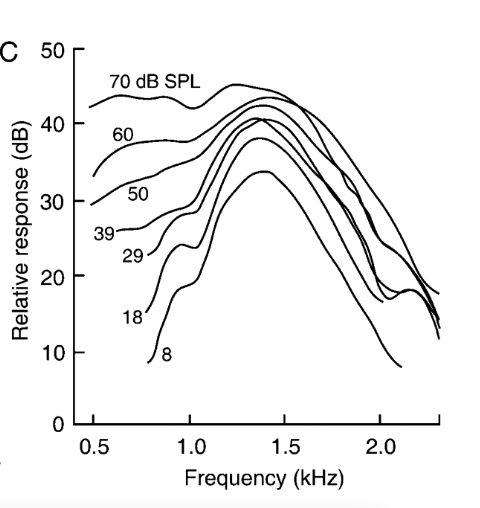
\includegraphics[width=0.5\textwidth]{auditory_system_FTC}
	\caption[Example of frequency tuning curve (FTC)]{Example frequency tuning curve (FTC) for a CF of approximately \qty{1.5}{\kilo\hertz}, and the impact of stimulus level on tuning (broadening of bandwidth and increase in upward spread of masking) \textbf{from pickles, no permission yet}.}
	\label{fig:auditory_system_FTC}
\end{figure}

The combined FTCs of all the ANFs innervating the cochlea results in frequency-dependent minimum acoustic level that can be detected by the auditory system. In the presence of background noise, the activation of the cochlea and subsequent firing of the corresponding ANFs due to the interfering noise obscures the firing due to the desired signal (i.e., spectral masking). This perceptual masking effect reduces audibility at the frequencies where noise is present, and raises the effective threshold of hearing. 


\subsection{Sound Localization}

The detection of the direction of arrival (DOA) and distance of sound sources plays an important role in everyday life. Not only is sound localization useful for spatial awareness, but there are several auditory mechanisms by which spatial information is used help with speech perception when in adverse listening conditions \citep[e.g., the cocktail party effect, reviewed by][]{bronkhorst2000cocktail}). A detailed review of the sound localization cues and physiology was provided by  \cite{risoud2018localization}, but has been summarized below.

Acoustic properties of the human auditory system enable sound localization by means of a number of binaural and monaural spatial cues. Firstly, when sound originates from a source to one side of the head, the acoustic level is attenuated on the other side due to reduction in direct line-of-sight propagation. This is referred to as the head-shadow effect and produces a difference in acoustic level between the ears called an interaural level difference (ILD). This effect is less pronounced at low frequencies (approximately below \qty{1960}{\hertz}), and most pronounced above approximately \qty{3}{\kilo\hertz}. ILD magnitude varies depending on individual head acoustics and horizontal angle of arrival (i.e., azimuth angle), and is one of the two spatial cues decoded by the brain to estimate azimuth DOA. The smallest perceiveable ILD has been shown to be approximately 0.5 -- 1 \unit{\decibel}.

Sound arriving from an off-axis azimuth angle will also arrive at the closer ear first, resulting in an interaural time delay (ITD). The auditory system estimates DOA from ITDs by analyzing phase differences between the ears. For wavelengths less than the distance between the two ears, multiple periods can occur within the time difference, resulting in an ambiguous mapping between phase difference and DOA. For this reason, ITDs become less reliable for frequencies above approximately \qty{1500}{\hertz}. In the case of complex amplitude modulation waveforms such as speech, the auditory system can use some higher frequency ITD information by tracking delays in the temporal envelope rather than the high frequency carrier. The shortest perceivable ITD has been shown to be around 10 \unit{\micro\second}.

For vertical location finding (i.e., sound localization on the elevation angle), the auditory system takes advantage of the acoustic characteristics provided by the shape of the outer ear. The exposed flange of the pinna has a complex shape with many different ridges which introduce acoustic reflections in the vicinity of the ear canal. These reflections and those provided by the head and upper body result in a DOA-dependent spectral coloration which is referred to as a head-related transfer function (HRTF). Spectral notches produced by destructive interference of head-related reflections are particularly used by the auditory system in estimation of the elevation angle. HRTF have been shown to be most reliable for frequencies above approximately \qty{7}{\kilo\hertz}

To estimate the distance of a sound source, the auditory system takes advantage of spectral cues and reverberation-related cues. In the presence of reverbant reflections, the listener first detects the direct sound (i.e., not reflected), and then receives a number of reflections dependent on the room acoustics. Due to the inherit attenation of acoustic signals as they propagate, as the separation between the sound source and the listener increases, the direct sound is attenuated and becomes increasingly dominated by the reflections. In this way, the auditory system is able to use an estimate of the direct-to-reverberant ratio to detect the distance of the sound source. Similarly, the time delay between the direct sound and the first reflections (i.e., the initial time delay gap, ITDG) decreases with distance, and can be used to estimate distance. Additionally, since higher frequency acoustic signals decay more rapidly over distance, the auditory system is able to use the lowpass-filtered quality of signal spectrum to estimate distance.

There are also several dynamic methods by which humans reinforce the spatial information decoded from the above described cues. Head turning is often performed instinctively to manually adjust spatial cues and confirm the changes that occur. Visual information is also incorporated both as a means of detecting and maintaing location estimates.

\section{Hearing Loss}

A detailed discussion of this topic can be found in \cite{pickles2013} and the review by \cite{shapiro2021hearing}, but the important concepts have been summarized here. 

\subsection{Overview of Hearing Loss}

Hearing loss has many causes and impacts, which are broadly grouped into three categories: Conductive, Sensorineural and mixed hearing loss. Conductive hearing loss describes any damage to the structures of the outer and/or middle ear. Sensorineural hearing loss describes any damage to the inner ear organs and auditory nerve, and is the most common type. Mixed hearing loss represents any combination of conductive and sensorineural hearing loss. Hearing loss can be in a single ear or in both ears (i.e., unilateral or bilateral), and can be symmetric or asymmeric between the two ears. Impairment may be present since birth (i.e., congenital hearing loss), or may accumulate over time (i.e., progressive hearing loss), or happen rapidly at some point in life (i.e., sudden hearing loss).

Conductive hearing loss includes blockages of the ear canal (e.g., due to ear wax build up), infections in the outer/middle ear, fixation of the ossicles, and damage to the tympanic membrane or oval/round windows. The general result of these issues is reduced energy transfer to the inner ear. Conductive damage can often be treated by medication or surgery, and otherwise is still easily treated by hearing aids since the inner ear is not affected and therefore the mapping/encoding of frequencies is not changed.

Sensorineural hearing loss can be caused by infection, aging, genetics, noise exposure, and most commonly results in damage or loss of stereocillia and hair cells in the cochlea. Hair cells and stereocilia are fragile and irreplaceable, and as will be described in the next section, loss of these structures significantly changes the neural encoding of sounds making it very hard to treat effectively. Age-induced sensorineural hearing loss (i.e., presbycusis) is thought to be caused by a combination of genetics and environmental factors. It is typically symmetric and bilateral, and primarily occurs at high frequencies. Chronic loud noise exposure primarily impacts frequencies in the \qty{3}{\kilo\hertz} to \qty{6}{\kilo\hertz} range, and is usually bilateral and symmetric, but may be asymetric if the exposure is asymmetric. Individual acoustic events of substantial loudness may also cause temporary or permanent damage to stereocilia (i.e., acute acoustic trauma). Mild trauma may only result in temporary damage, while more severe trauma are more likley to permanently bend or break stereocilia resulting in complete loss of transduction. The stereocilia of OHCs are more likely to be lost completely, while IHCs tend to only lose some stereocilia resulting in some transduction remaining with weaker sensitivity. Since sensorineural hearing loss largely impacts the auditory system on a per-hair cell basis, and since hearing aids process the acoustic signal before transimission into the cochlea, the efficacy of hearing aids at compensating these impairments is somewhat limited.

Hearing loss may also be induced by medications with ototoxic effects, which describe a wide range of biochemical reactions with various parts of the auditory system. Most often this begins with fusion or loss of stereocilia, eventually resulting loss of hair cells. Examples of ototoxic medications include many chemotherapies and antibiotics.

\subsection{Perceptual Impacts of Sensorineural Hearing Loss} \label{section:hearing_loss_impacts}

When sensorineural hearing loss impacts OHC function, this usually results in reduction of the active amplification mechanism provided by the electromotility of the OHCs. This and the reduction of IHC sensitivity produces reduced excitation at the auditory nerve. This results in an increase in the threshold of hearing, which can have a significant impact on audibility at conversational speech levels. 

The loss of the active amplification provided by OHCs also results in a reduction in the non-linearities of the auditory system. The dynamic range compression provided by these non-linearities is crucial for the perception of the wide dynamic range of environmental sounds. As a result, individuals with sensorineural hearing loss tend to lose perception of quiet sounds, but still perceive louder sounds at the same level. In other words, the dynamic range between audibility of quiet sounds, and discomfort of loud sounds, is less for individuals with sensorineural hearing loss. An additional related effect is an increased rate of change in perceived loudness with respect to acoustic stimulus level, which is referred to as loudness recruitment. These issues motivate the usage of wide dynamic range compression (WDRC) algorithms for hearing aid amplification instead of linear gains \citep{dillon2012hearing}. If linear gains are used and set high enough to make quieter sounds audible, this would make louder sounds uncomfortably loud.

Additionally, the loss of OHC function results in loss of the sharp tuning of the auditory ANFs. This results in a broadening of the ANF tuning and reduces the frequency resolution of the cochlea. 

A reduction in temporal sensitivity has also been correlated to both aging and sensorineural hearing loss. The physiological explanations for these effects are complex and still under study, but it is generally explained by reduced ability to track the temporal fine structure (TFS) in complex broadband stimuli, especially in the presence of noise \citep{xia2018effects}. There are a number of proposed physiological explanations for this including a reduced number of ANFs, reductions to phase locking of neurons with periodic waveforms, the broadening of cochlear tuning resulting in more complex waveforms arriving at each ANF, and distorted basilar membrane phase response  \citep{tsironis2024adaptation}.

The reduction of spectral and temporal resolution results in a coarse and distorted neurological encoding of sound, which significantly impacts speech perception (i.e., impairs the classification of phonemes, as will be described later). In addition, loss of temporal resolution impairs the ability of the auditory system to track ITDs which has a significant impact on sound localization.

\section{Speech Production}

The ability of humans to generate speech sounds is central to our social communication and societal organization. Speech communication is fasciliated by manipulating the body to generate audible sounds from the mouth and/or nose. A specific configuration of the speech-related physiology produces a specific sound which is referred to as a phoneme. Phonemes are produced together to form words, which are spoken in sequence to form sentences. By inversely mapping acoustic signal properties to the speech-related configuration used to produce them, listeners are able to decode the intended sentence and perceive its meaning.

A detailed discussion of this topic can be found in \cite{quatieri2002discrete}, but the important details have been summarized here.

\subsection{Anatomy of Speech Production}

The physiology underlying speech production can be braodly broken down into three sections: The lungs, the larynx and the vocal tract. The lungs act as a power supply, contracting and expanding to provide air pressure to the larynx. The larynx uses the power from the lungs to generate a specific of acoustic waveform. The vocal tract shapes the acoustic waveform before its emission from the mouth and/or nasal passage. 


\begin{figure}[H]
	\centering
	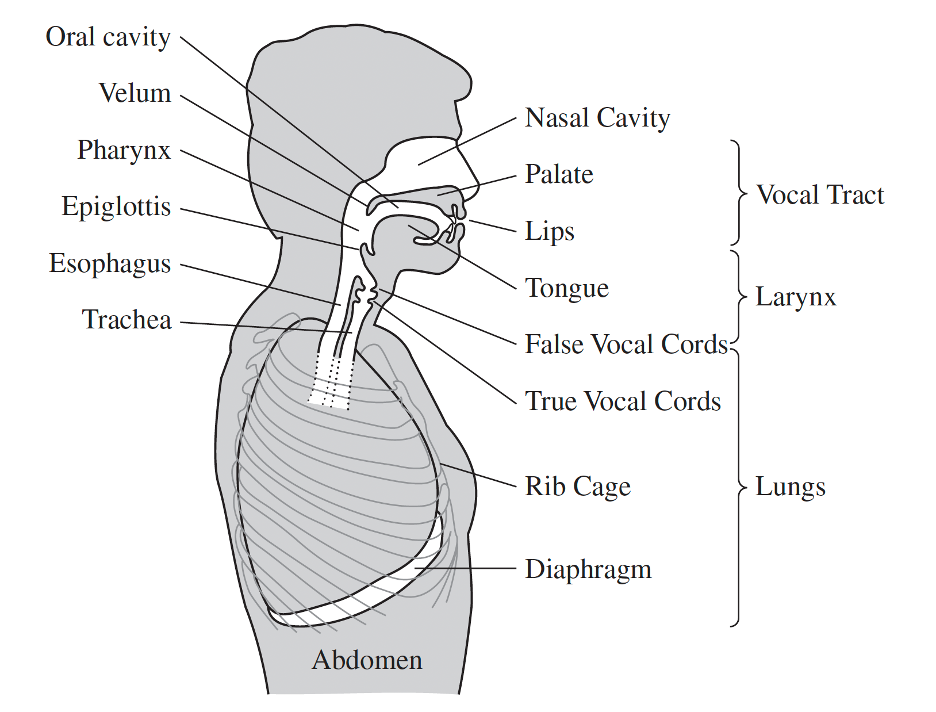
\includegraphics[width=0.7\textwidth]{speech_production_system}
	\caption[Human speech production system]{Human speech production system. \textbf{from quatieri, no permission yet}.}
	\label{fig:speech_production_system}
\end{figure}

Inside the larynx, air flow into the vocal tract is controlled by opening and closing three separate muscle-controled barriers: the false vocal folds, the true vocal folds, and the epiglottis. The vocal folds are composed of two masses of flesh which can be pulled towards the sides of the sides of the larynx revealing a opening known as the glottis (i.e., glottal slit). Muscles-activated control over both the size of the glottis and the tension in the vocal folds give rise to three different modes of operation: breathing, voicing and unvoicing. When the glottis is fully open, the lungs push air into the vocal tract with minimal resistance (i.e., breathing). When the glottis is closed slightly and pulled tight, the applied air pressure initiates an periodic pattern of glottal opening and closing (i.e., glottal pulsing). This process releases a periodic acoustic waveform into the vocal tract (i.e., voicing). The pitch period of voiced speech is controled by tightening and loosening the vocal folds. During unvoicing, the glottis is left open similar to breathing, but the folds are pulled tighter generating audible turbulence. Unvoicing is used in the speech sounds such as the ``h" in ``house"

The vocal tract is an oral cavity extending from the larynx to the lips and nasal passage. Manipulation of the position of the tonge, lips and mouth changes the acoustic resonances of the cavity to modulate the spectral shape of the emitted acoustic waveform. These resonances, called formants, emphasize certain harmonics of the glottal pulse waveform. The relative positioning of formants is central to the classification of different voiced phonemes (e.g., ``a", ``e", ``o"). When the lips or tonge are used to seal the mouth during voiced speech, the glottal pulsing waveform is forced through the nose, generating nasal phonemes (e.g., ``ng" in ``sing", or ``m" in ``mother"). Applying pressure behind the lip or tonge seal before releasing it produces a sudden burst of air from the mouth, generating an impulsive sound known as a plosive phoneme (e.g., ``p" in ``pop", ``t" in ``train" or ``c" in ``cane"). When the lips or tonge are positioned to provide a partial seal of the mouth, an audible turbulance is produced which is classified as a fricative phoneme (e.g., ``sh" in ``she" or ``s" in ``snake"). 

\subsection{Classification of Speech Sounds}

Together the voicing state of the glottis (i.e., voiced, unvoiced or breathed) and the vocal tract configuration (i.e., formant ratios, fricatives, plosives, nasals) form a collection of acoustic cues which are used by the listener to interpret what is being said.  The interaction between each of these speech parameters forms a much wider set of phonemes. Vowels are voiced phonemes with no frication or obstruction of the vocal tract (e.g., ``a" in ``apple"). Fricatives can be unvoiced (e.g., ``f" in ``flake") or voiced (e.g., ``v" in ``van"). Plosives can be unvoiced (e.g., ``p" in ``pop") or voiced (e.g., ``b" in ``boot"). Diphthongs, liguids and glides are all characterized by a time-varying vocal tract between vowels (e.g., ``y" in ``boy"). Affricatives are describe the time-varying transition between plosives and fricatives (e.g., ``ch" in ``chew").

\subsection{Discrete-Time Speech Production Model} \label{dt_speech_model}

The process of speech production can largely be described with a source-filter model. The acoustic waveform generated by the lungs and larynx are modeled as a source, which is processed by a filter which models the vocal tract and acoustic raditation from the lips. A complete discrete-time model of this process is shown in Figure \ref{fig:dt_speech_production_model}.

\begin{figure}[H]
	\centering
	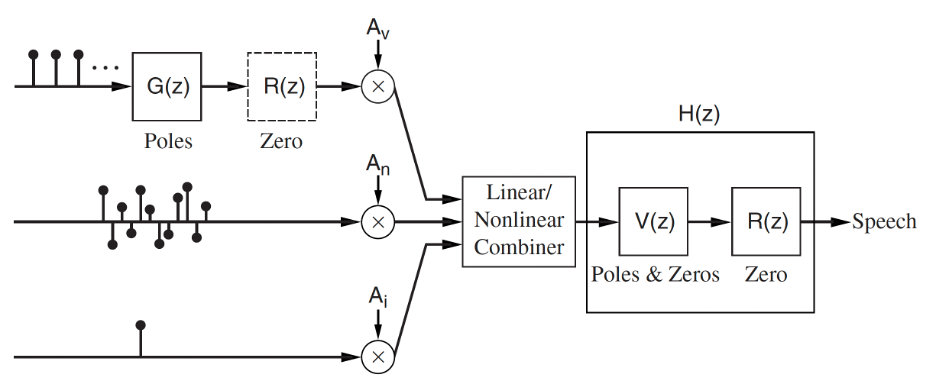
\includegraphics[width=\textwidth]{dt_speech_production_model}
	\caption[Discrete-time speech production model]{Discrete-time speech production model. \textbf{from quatieri, no permission yet}.}
	\label{fig:dt_speech_production_model}
\end{figure}

In this paradigm, the lungs and larynx are grouped into an idealized source model which generates a combination of idealized source signals depending on voicing mode:

\begin{eqnarray}
	u_\mathrm{g}(n)=\sum_{k=-\infty}^{\infty} \delta(n-kP) \\
	u_\mathrm{i}(n)=\delta(n) \\
	u_\mathrm{n}(n)\sim\mathcal{N}(0,1)
\end{eqnarray}


\noindent
where $u_\mathrm{g}(n)$ represents idealized glottal pulsing during voiced phonemes, $u_\mathrm{i}(n)$ represents idealized inpulsive bursts during plosive phonemes, and $u_\mathrm{n}(n)$  representation idealized turbulance during fricative phonemes. 

To obtain an accurate model of the glottal pulse train waveform, the idealized impulse train $u_\mathrm{g}(n)$ is convolved with an individual cycle of glottal pulsing. The Z-transform of a typical glottal flow waveform can be modeled by two identical poles outside the unit circle (i.e., two maximum phase poles representing a left sided sequence).

\begin{equation}
	G(z)=\frac{1}{(1-\beta z)^2} \qquad \beta<1 \label{eq:glottal_pulse_z}
\end{equation}


Therefore the Z-transform of the glottal pulse train modeled is $U_\mathrm{g}(z)G(z)$, and the Z-transform of the overall source model is

\begin{eqnarray}
	U(z)=A_\mathrm{v} U_\mathrm{g}(z) G(z)+A_\mathrm{i} U_\mathrm{i}(z)+A_\mathrm{n} U_\mathrm{n}(z)
\end{eqnarray}

During oral voiced speech, it has been shown that the vocal tract effect can be modeled by a minimum-phase all-pole filter \citep{atal1971speech}. However, when the oral tract is sealed by the tonge or lips (e.g., during nasalized phonemes) and during unvoiced speech, the effective filter has been shown to have some mixed-phase zeros. Therefore a complete model for the vocal tract is a mixed-phase filter with poles and zeros, i.e.,

\begin{eqnarray}
	V(z)=
	\frac
	{\prod_{k=1}^{M_{\mathrm{min}}}(1-\tilde{b}_{\mathrm{min},k}z^{-1}) 
		\prod_{k=1}^{M_{\mathrm{max}}}(1-\tilde{b}_{\mathrm{max},k}z^{-1})}
	{\prod_{k=1}^{N_{\mathrm{min}}}(1-\tilde{a}_{\mathrm{min},k} z^{-1})}
\end{eqnarray}

The acoustic radiation from the lips (i.e., the radiation impedance) imparts a highpass response which can be approximately modeled by a single zero just inside the unit circle, i.e.,

\begin{equation}
	R(z)\approx 1-\alpha z^{-1} \qquad \alpha <1
\end{equation}

Therefore the complete filter model is $H(z)=V(z)R(z)$, and the complete source-filter model of speech production is

\begin{equation}
	S(z)=U(z)H(z)
\end{equation}

It is also common to group the Z-transform of the glottal pulse waveform, $G(z)$, into the filter model so the source can always be treated as an idealized uncorrelated excitation (i.e., impulse train, impulse or white noise). In this case the speech production filter, $H(z)$, has mixed-phase poles and zeros.

\begin{equation}
	H(z) = G(z)V(z)R(z) = 
	\frac
	{\prod_{k=1}^{M_{\mathrm{min}}}(1-\tilde{b}_{\mathrm{min},k}z^{-1})
		\prod_{k=1}^{M_{\mathrm{max}}}(1-\tilde{b}_{\mathrm{max},k}z^{-1})}
	{\prod_{k=1}^{N_{\mathrm{min}}}(1-\tilde{a}_{\mathrm{min},k} z^{-1})
		\prod_{k=1}^{N_{\mathrm{max}}}(1-\tilde{a}_{\mathrm{max},k} z^{-1})}
\end{equation}

From the geometric series expansion, it can be shown that a single zero inside the unit circle can be represented by a set of infinite poles inside the unit circle, i.e.,

\begin{equation}
	1-\tilde{b}z^{-1} = \frac{1}{\prod_{k=0}^{\infty}(1-\tilde{a}_k z^{-1})}, \;\; |z| > |a| \label{eq:zero_approx}
\end{equation}

\noindent
and in practice, a sufficiently large finite number of poles works with reasonable accuracy. Therefore an all-pole, i.e., autoregressive (AR), model of speech production is often used. i.e.,

\begin{eqnarray}
	H(z) = \frac{A}{\prod_{k=1}^{p}(1-\tilde{a}_k z^{-1})} = \frac{A}{1 - \sum_{k=1}^{p} a_k z^{-k}}\\
	S(z)=U(z)H(z) \\
	s(n) = \sum_{k=1}^{p}a_k s(n-k) + A u(n) \label{eq:AR_speech}
\end{eqnarray}

It is important to note that this stationary model of the speech production system is incomplete when in comes to modeling full utterances that span multiple phonemes, or even phonemes that involve time variance in the vocal tract (e.g., diphthongs). To address this, the source weights ($A_\mathrm{v}$, $A_\mathrm{i}$ and $A_\mathrm{n}$) and the filter parameters must all be made time-varying.

\section{Speech Perception in Reverberation}

\subsection{Characterizing Speech Perception} \label{section_perception}

As a whole, speech perception describes a listener's ability to hear and understand what is being said by a talker. This is directly dependent on the listener's ability to detect the presence of the acoustic speech signal, and decode the speech cues to accurately reconstruct the spoken utterances. There are several characteristics of speech perception which are related but distinct: speech audibility, speech intelligibility and listening effort.

Audibility describes the listener's ability to detect the presence of sound. The auditory system is physically capable of detecting any sound that is above the absolute threshold of hearing. As such, speech audibility may be defined as the fraction of speech content over time that is above the listener's threshold of hearing.

Speech intelligibility (SI) describes how accurately the listener is able to identify what is being said, and is usually measured as a fraction of phonemes or words correctly identified. SI is typically evaluated based on objective tests involving human participants. Speech is presented, and the participant attempts to identify what is being spoken. Sometimes nonsense utterances are used to remove effects of lexical knowledge. 

\begin{equation}
	\mathrm{SI} = \frac{\mathrm{Correctly \; Identified \; [words/syllables/phonemes]}}{\mathrm{Total \; Presented \;  [words/syllables/phonemes]}}
\end{equation}

Listening effort (LE) describes the allocation of mental resources required to understand speech. When speech cues are obscured (e.g., in noisy or reverberant environments), the brain has to work harder to fill in missing information (i.e., post-diction). LE is often evaluated by presenting a test signal to participants and asking them to complete an effort-related questionnaire, but in general it is too complex to evaluate in a single test. It has been proposed that a more statistically consistent evaluation of listening effort is based on three separate factors \citep{shields2023exploring}: self-reported LE, behavioral signs of LE, and physiological signs of LE. Self-reported LE is usually evaluated by having particpants complete questionairres assessing their effort during listening, and fatigue after listening. Behavioral signs of LE describe reduced ability to complete mentally-intensive tasks due to exhaustion, and is assessed by evaluating their performance on a selected test task. Physiological signs of LE are widespread and can be assessed via objective biological measurements such as electroencephalogram analysis (EEG), functional magnetic resonance imaging (fMRI), eye tracking and heart rate tracking. Increased listening effort in every day life can have psychological effects such as distress or fatigue and has been shown to lead to social withdrawal and to increase with prevalence of stress-related leave from work \citep{ohlenforst2017effects}. Although speech intelligibility and listening effort are closely related, an increase listening effort is not always correlated to a decrease in speech intelligibility \citep{winn2021listening}.

When evaluating the performance of a speech reproduction system such as a hearing aid, speech quality is also an important consideration in the subjective experience of the user. Speech quality (SQ) is usually evaluated based on subjective ranking of a test/distorted signal on a provided scale.  The most common test is the so-called mean opinion score (MOS) test in which the participants are asked to rank the quality of a test signal on a five point scale (i.e., absolute category rating, ACR). The MOS test procedure consists first of a training phase (i.e., anchoring phase) where the participant is presented with example signals for the low, middle and high quality categories. After the training phase, the evaluation phase is completed using the real test signal. The test is repeated for a group of participants, and the MOS rating is computed as the average ACR accross all participants. An alternative quality test is the comparative mean opinion score (CMOS) where the participants are presented with a test signal and a separate clean reference signal, and are asked rank how much better or worse the quality of the test signal is relative to the reference signal.

\subsection{Neural Encoding of Acoustic Speech Cues} \label{section:encoding_acoustic_cues}

%The acoustic cues that are exploited by the auditory system to perceive speech can be categorized as spectral cues and temporal cues. Spectral cues

Complex broadband speech signals can be modeled as a superposition of narrowband amplitude modulation signals. In each of these bands the high frequency carrier information is referred to as the temporal fine structure (TFS) and the amplitude modulation is referred to as the envelope (ENV). The cochlear filters in the auditory system perform this narrowband signal decomposition, and the TFS/ENV acoustic cues are encoded into the neural representation and are analyzed to percieve speech. TFS acoustic cues are primarily encoded into the precise ANF spike-timing due the phase-locking of spiking to the carrier. Since ANF phase-locking breaks down for frequencies over 4 -- 5 \unit{\kilo\hertz}, the neural encoding of TFS is only effective at lower frequencies. TFS acoustic cues provide information on details such as the pitch/periodicity and harmonics of of the signal, formant transitions, and timing information for sound localization. ENV acoustic cues are encoded mainly in fluctuations to the ANF firing rate and in the phase-locking of ANF spiking to the amplitude modulation phase which occurs at higher frequencies. ENV cues provide information on speech amplitude fluctuations, unvoiced fricatives, voiced/unvoiced segment detection and syllable/word onset and stop detection. Although harmonic/formant information is described by TFS acoustic cues, ENV cues are analyzed on a per auditory filter basis, thus also providing spectral information such as formant locations and spectral tilt.

ENV acoustic cues are generally described as varying at rates of less than 20 -- 50 \unit{Hz}, while TFS acoustic cues vary at much higher carrier frequency rates. Moreover, word/syllable rates described by ENV cues are even slower, having periods of around 250 -- 500 \unit{\milli\second} (i.e., 2 -- 4 \unit{\hertz}). ENV acoustic cues also have a much larger dynamic range than TFS cues.

It is well understood that in quiet environments ENV cues provide sufficient information for to maintain intelligibility and that TFS cues play a more significant role in noisy/reverberant environments \citep{shannon1995speech, smith2002chimaeric}. It has been shown that full intelligibility can be achieved in quiet for noise vocoded speech because phonemes can be identified from the spectral information encoded into ENV cues on a per frequency band basis. In noise vocoded speech, only the perception of pitch/harmonics/sound localization is lost which are note crucial for intelligibility in quiet. However, it has also been shown that TFS cues play a key role in intelligibility in noise, and that in quiet they still play an signficant supportive role which impacts LE \citep{wirtzfeld2017predictions}. The mean-rate information of ANF spike patterns has been shown to primarily represent ENV acoustic cues on a per-CF basis (i.e.,temporal envelope and formants), while the fine ANF spike-timing information encodes TFS acoustic cues (i.e., pitch, harmonics and timing information).

At higher sound pressure levels and for hearing impaired listeners, TFS cues can be severely distorted by the broadening of auditory filter tuning, upward spread of masking and reductions in ANF phase-locking. ENV cues are also distorted but are much more robust due their slower time-variance which does not require as precise time resolution and due to their broadband nature not requiring as precise frequency resolution. Since higher sound pressure levels have a severe negative impact on the encoding of TFS cues, using a linear hearing gain to compensate speech audibility will not be effective at restoring TFS cues. Conversely, the robustness of ENV cues to these distortions makes them easier to restore by linear amplification. Additionally, since full intelligibility can be acheived from ENV cues alone, distortions of TFS cues at higher gains does not impact intelligibility (in absense of noise and reverberation). However, distortions to TFS cues will still have a negative impact on LE and there additionally still exists a trade off between audibility and listener comfort. This will be discussed more later on.


\subsection{Impact of Reverberation on Speech Cues} \label{reverb_impact_speech_cues}

As previously discussed, phoneme recognition relies on the identification of acoustic cues. Temporal cues such as periodicity, onsets, offsets and stops are important to detect the boundaries of words and identify phonemes as voiced, fricative and plosive. Spectral cues such as phoneme ratios and spectral tilt are important to differentiate specific voiced phonemes. Accurate phoneme identification therefore is strongly dependent on tem. 

Reverberation smears energy accross time, blurring temporal and spectral cues. Periods of low energy are filled with reverberant energy, smoothing out temporal envelope, thus blurring word onsets, offsets and stops. Phonemes also overlap in time, resulting in a masking effect.  Speech perception is particularly impacted during highly time-varying speech segments (e.g., consonants or word boundaries) and following loud bursts which take longer to decay. Formant transitions during diphthongs, liguids and glides are also flattened making them harder to identify.

\subsection{Impact of Reverberation on Speech Intelligibility and Listening Effort} \label{section:reverb_si}

It has been shown that reverberation and noise both have a negative impact on speech intelligibility and listening effort. However, in most realistic listening environments, where reverberation time is fairly short and SNR is positive, the effects on speech intelligibility are minimal \citep{schepker2016perceived}. This can be explained by the fact that the higher time-variance and smaller dynamic range of TFS acoustic cues makes them more sensitive to reverberation than ENV acoustic cues. Since ENV acoustic cues are generally more crucial for intelligibility, signficant reverberation energy and long reverberation times are required to obscure ENV cues and thus negatively impact intelligibility. Conversely, even small amounts of reverberation distort TFS cues thus impacting listening effort.

Normal hearing listeners are generally able maintain good speech undestanding even under reasonably severe listening conditions \citep{schepker2016perceived} due largely to perceptual adaptations which will be explained in the next section. This is especially true when the listeners has prior exposure to the listening environment \citep{george2010measuring}.

Hearing impaired individuals are more sensitive to the effects of reverb and noise. Even when audibility is good, intelligibility and listening effort tend to be worse due to degraded temporal and spectral resolution from sensorineural hearing loss \citep{reinhart2018listener} and reduced perceptual adaptations \citep{srinivasan2017role, roberts2003effects}. There is a lot of variability in the impact of reverberation for hearing impaired listeners, and the reasons are not fully understood. However it has generally been shown that more severe impairment equates to more difficulty in reverberant environments \citep{xia2018effects}.

The individual and combined impacts of reverberation and noise are often investigated through from the perspective of speech transmission index (STI). This is done by mapping both variables onto a 2D grid showing iso-STI contours (e.g., Figure \ref{fig:equal_sti_contours}). In this way the impacts of reverberation and/or noise can be analyzed through a single variable. STI has been shown to be correlated to speech intelligibility and listening effort regardless of whether the changes in STI are due to reverberation or noise.

\begin{figure}[H]
	\centering
	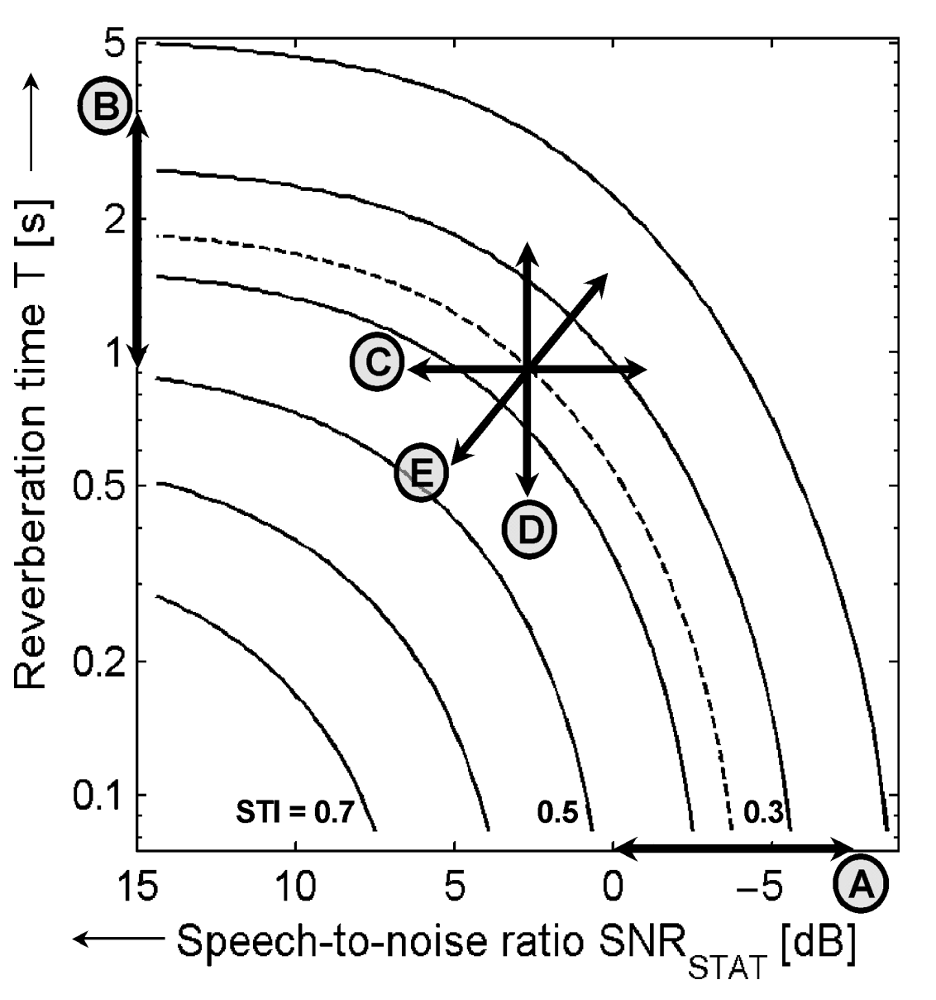
\includegraphics[width=0.5\textwidth]{EqualSTIContours}
	\caption[Mapping of SNR/T60 to STI]{Mapping of SNR and reverberation time (synthetically generated exponentially decaying Gaussian RIRs) to STI. The dotted contour denotes the speech recongition threshold (SRT). \textbf{from George et al, no permission yet}.}
	\label{fig:equal_sti_contours}
\end{figure}

For normal hearing listeners, \cite{george2010measuring} showed that the minimum conditions for \qty{50}{\percent} speech intelligibility (i.e., the speech recognition threshold, or SRT) is approximately an STI of 0.36, which is represented by the dotted contour in Figure \ref{fig:equal_sti_contours}. This translates to a reverberation time of approximately \qty{2}{\sec}, or a SNR of approximately \qty{-4}{\decibel}, which are very severe conditions not typically experienced in everyday life. As the conditions improve from this point (i.e., as reverberation time decreases and/or SNR increases), speech intelligibility very rapidly returns to \qty{100}{\percent}. This shows the insensitivity of speech intelligibility as a measurement of the impacts of reverberation under typical conditions.

Conversely, listening effort has been shown to vary monotonically with reverberation time and noise even under moderately severe conditions. For this reason, listening effort is generally considered a better metric under typical listening conditions, and a combination of listening effort and speech intelligibility is best for a reliable analysis over a wide range of conditions \citep{schepker2016perceived}.

Independent of hearing loss, other factors such as age related neurological/auditory deteriorations and differences in working memory capacity have been shown to impact the extent to which reverberation inhibits speech perception \citep{reinhart2018listener}.

\subsection{Impact of Reverberation on Spatial Cues} \label{section:reverb_spatial_cues}

As perviously discussed, detection of the directional of arrival (DOA) of sound is important for spatial awareness and speech perception. In anechoic environments, sound arrives from a single distinct direction, making localization a relatively simple task. In reverberant environments, sound arrives from many directions due to reflections, which blurs the spatial cues which are central to sound localization (i.e., ILDs, ITDs and HRTFs).

However, It has been shown that with extended exposure to a reverberant environment, the auditory system's ability to estimate direction and distance improves greatly. This is due to perceptual adaptations which are described in the next section.

\subsection{Perceptual Adaptation to Reverberation and Noise} \label{perceptual_adaptations}

Normal hearing (NH) auditory systems have a strong ability to maintain speech perception in adverse listening conditions due a number of perceptual adaptations which work to provide phonetic perceptual consistency. A detailed overview of these perceptual adaptations can be found in the review by \cite{tsironis2024adaptation}, but the key information is summarized below.

\subsubsection{The Precedence Effect}

The precedence effect (PE) describes a perceptual phenomena whereby delayed repitions of the same sound are perceived as an individual sound, provided the delay between the sounds is short enough. This effect was originally demonstrated by \cite{wallach1949precedence} and \cite{haas1951einflubeta} and was reviewed by \cite{litovsky1999precedence}. Studies of the percedence effect usually involve playing two identical stimuli with a delay between them (i.e., a lead-lag pair). Commonly clicks are used but studies have also been done involving more complex stimuli such as noise and speech. The precedence effect is most pronounced for brief/transient sounds such as clicks but is still reasonably effective for complex stimuli like speech. The effect is much weaker for stationary sounds such as sustained tones. 

Under the umbrella of the precedence effect there are three phenomena which are separate but related: Lead-lag fusion, lead-lag localization dominance, lead-lag discrimination suppression. 

Lead-lag fusion describes the process whereby lead-lag pairs of stimuli are perceived as a single auditory event provided the delay between the stimuli is less than the so-called echo threshold (i.e., the echo fusion threshold). This results in a sort of echo suppression for reverberation whereby reflections that arrive within the echo threshold are fused with the direct sound. Reflections with delays greater than the echo threshold are perceived as distinct and have an adverse affect on speech perception. Echo thresholds are typically in the range of \qty{5}{\milli\sec} to \qty{30}{\milli\sec}, but can be as low as \qty{2}{\milli\sec} or as high as more than \qty{100}{\milli\sec}. This wide range is dependent on stimulus characteristics (i.e., spatial, spectral and temporal properties) and the listener's age, hearing status and extent of prior exposure to the current room acoustics. Lead-lag fusion has been shown to occur even when the lagging stimulus is up to 10 to 15 \unit{\decibel} louder than the leading stimulus. 

Lead-lag localization dominance is a phenomena whereby the fused signal is perceived to arrive from or near the direction of the leading stimulus. Lead-lag discrimination suppression describes the listener’s inability perceive the location of the lagging stimulus. Together, localization dominance and discrimination suppression are responsible for reducing disruptions to sound localization due to reflections in reverberant environments. Although fusion occurs for delays lower than the echo threshold, localization dominance and discrimination suppression only occur for shorters delays. Additionally, for very short delays less than approximately 0.5 to 1 milliseconds, localization dominance and discrimination suppression break down, and summation localization occurs. For these delays, sound is perceived to arrive from the average direction between the leading and lagging stimuli (i.e., weak precedence).

The precedence effect also includes an adaptive mechanism called the build-up effect. When lead-lag pairs are repeated, over time the echo threshold has been shown to increase, resulting in fusing of longer and longer delays with the direct sound. As a result, when a listener is exposed to stimuli in a relatively stationary acoustic environment, their ability to perceptually suppress reverberant reflections increases over time. This is an example of how normal hearing individuals benefit from prior exposure to room acoustics. Conversely, when room acoustics change, this can result in a mismatch between the lead-lag relationships mapped by the auditory system and the true characteristics of the acoustic reflections. In this situation, the mechanisms of the precedence effect reset to their base states, and the listeners perceives an increase in amount of echo. This is referred to as the breakdown effect.

Hearing impaired listeners have been shown to experience less of the benefits of the precedence effect \citep{roberts2003effects, rennies2022spatio}. Research into the physiological explanations for this is ongoing, but it is generally thought to be related to reduction of temporal resolution in impaired auditory systems. This contributes to the difficulties hearing impaired listeners experience in reverberant environments.  

\subsubsection{Spatial Release From Masking} \label{section_srm}

Another key perceptual adaptation involved in handling adverse listening conditions is spatial release from masking (SRM), which was reviewed by  \cite{litovsky2012spatial}. This phenominon encompasses several mechanisms by which the auditory system leverages the spatial diversity between the ears to process spatially separated sound sources. In the presence of many interfering acoustic signals, a normal-hearing auditory system has a strong ability to isolate the target talker and maintain speech perception. This phenomena was originally explored by \cite{cherry1953some}, who referred to it as the ``cocktail party effect", and has since been largely attributed to SRM. Since this effect leverages spatial diversity, speech perception is better in noisy environments if the maskers are separated spatially (i.e., not co-located). 

There are three main mechanisms involved in SRM: The better ear effect, the binaural squelch effect and binaural summation. The better ear effect describes how the auditory system will increase focus on a single ear, chosen based on SNR estimated from ILD cues. It is well known that sounds arriving from one side of the head can be attenuated by up to approximately \qty{9}{\decibel} on the other side of the head due to the so-called head shadow effect. The binaural squelch effect (i.e., binaural unmasking) describes how the auditory system uses binaural cues to focus on the target. This effect is similar to beamforming in signal processing theory. Lastly, binaural summation is a mechanism whereby binaural listening improves perception of a target that is co-located with its masker. This is distinct from the binaural squelch effect in that it does not depend on binaural cues, and is more similar to signal averaging for noise reduction in signal processing theory. The better ear effect has been shown to be the most significant contributor to SRM, while the binaural squelch effect is less significant, and binaural summation is the least significant.

In a normal-hearing auditory system, SRM has been shown to provide from SNR improvements ranging from several \unit{\decibel} to upwards of \qty{25}{\decibel}. The benefits of SRM are much less for hearing impaired listeners, which is generally attributed to degraded binaural sensitivity caused by reduced temporal resolution. 

In reverberant environments, binaural cues are distorted, which reduces the effects of SRM. Generally, it has been shown that the benefits of SRM diminish as reverberation time increases. However SRM can also provide a small amount of reverberation reduction by suppressing the spatial directions corresponding to reflections. To explain this \cite{leclere2015speech} proposed a distinction between conventional binaural unmasking which reduces the effects of noise maskers, and binaural dereverberation which reduces the effects of self-masking due to reverberation. Binaural unmasking has been shown to be negatively impacted by reverberation, and interestingly binaural dereverberation has been shown to be negatively impacted by the presence of noise maskers.

%\section{Hearing Aids}
%
%Maybe later:
%- Might need to discuss practical requirements (delay etc)
%- Impact of acoustic design/positioning of hearing aids  (BTE, RIC, ITE etc) on spatial cues etc
%--> How hearing loss makes cues worse but hearing aids maybe make them doubly worse (often doesnt compensate spatial cue loss or even makes them worse)
%- How algorithms dont help the fundamental issues with hearing loss (especially relating to reverb)

\section{Metrics of Speech Perception}

As previously discussed, it has been shown that a combination of speech intelligibility and listening effort is best for evaluating the impacts of reverberation on speech perception under a wide range of acoustic conditions. Additionally speech quality is an important consideration in the subjective experience of hearing aid users.

While evaluations of SI, LE and SQ involving test participants are the most effective, they are time consuming and often not practical. A number of objective prediction metrics have been developed to estimate SI, LE and SQ by quantitative signal analysis. Although these prediction metrics are only approximations, many of them have proven to be strongly correlated to the true test metrics under certain conditions, and they are easily repoducible and greatly reduce the time required to evaluate speech reproduction systems such as hearing aids. 

When selecting a prediction metric for a study, careful attention must be given to ensure that the metric is suitable for the test conditions and the processing performed by the system under test (SUT). Since this thesis is focused on speech perception of hearing aid users in reverberant environments, it is important to include metrics that incorporate some modeling of the auditory system and the impacts of hearing loss (i.e., audibility, frequency tuning and non-linearities). If the metric does not include any modeling of the non-linearities in the human auditory system, it will not accurately predict the target speech perception metric accross a wide range of input levels, under non-linear distortions or under non-linear hearing aid processing such as dynamic range compression or statistical time frequency masking. Additionally, it is important to include binaural metrics that are capable of representing the perceptual adaptations that are key to speech perception in reverberant environments (i.e., the precedence effect and SRM).

\subsection{Objective Predictors of Speech Intelligibility} \label{section_si_metrics}

Objective predictors of SI generally consist of a signal analysis procedure which generates an intelligibility-related metric, and often provide a function that maps this objective metric to a prediction of subjective SI. Since the mapping between objective metrics and subjective SI ratings varies depending on the SI metric definition (e.g., phonemes or words identified correctly) and due to other factors such as participant knowledge of context, the mapping function is usually separate from the objective metric itself. The mapping is often non-linear due to floor and ceiling effects at 0\% and 100\% intelligibility respectively.

One of the earliest objective predictors is the articulation index (AI) \citep{kryter1962methods} which estimates intelligibility from audibility by analyzing SNR across frequencies. Under the assumption that speech has a dynamic range of approximately \qty{30}{\decibel}, if SNR (plus \qty{15}{\decibel} to get maxima of dynamic range) is greater than \qty{30}{\decibel} at all frequencies, all speech cues are assumed to be audible, and therefore intelligibility is assumed to be perfect. AI splits the noise and speech spectra into bands that roughly approximate human auditory filters and for each band specifies a lower and upper SNR limit corresponding to 0\% and 100\% audibility respectively (i.e., the articulation window). The AI metric is computated as the percentage of the articulation window covered, with frequencies weighted by perceptual importance.

The speech intelligibility index (SII) \citep{ansi1997methods} was provided as an extension of and replacement for AI. SII defines a generic framework for specifying signal spectrum levels, noise spectrum levels, hearing thresholds, and the measurement reference point (e.g., free field or ear drum). Additionally, it includes some simplistic modeling of the non-linearities of the auditory system, namely the upward spread of masking which occurs at higher acoustic levels. SII is calculated as:

\begin{equation}
	\mathrm{SII} = \sum_{i=1}^{n}I_iA_i
\end{equation}

\noindent 
where $i$ is the frequency band index, $n$ is the number of bands, $I_i$ is a frequency weighting function and $A_i$ is an audibility function. The frequency weighting is selected to represent the perceptual importance of different frequencies.  The audibility function is calculated as the per-band ratio of SNR to \qty{30}{\decibel} to represent the fraction of speech cues in \qty{30}{\decibel} dynamic speech that are audible. Finally the SII is limited to values ranging from 0 to 1. The speech and noise spectra are often pre-processed with a spectral weighting that better represents perceptual loudness / frequency dependent thresholds of hearing \citep[e.g., A-weighting which approximates 40-phon equal-loudness contour, ][]{iec2003Aweighting}, and can be weighted differently to model hearing loss. 

The speech transmission index (STI) \citep{iec2003sti} modified SII to estimate intelligibility by measuring changes to the spectrum of the temporal envelope rather than SNR. STI is based on the concept of the so-called modulation transfer function (MTF) which measures the ratio of temporal envelope per-bin from the input to the output of an acoustic channel. Specific narrowband test signals are used to measure MTF in octave frequency bands for a range of modulation frequencies. The STI metric is calculated by averaging over modulation frequencies, and performing a perceptually-weighted average over frequency bands. The calculation includes adjustments for auditory thresholds, noise levels and upward spread of masking. STI has been shown to have a strong correlation to SI under reverberation \citep{schepker2016perceived}.

Although STI and SII are correlated to SI, they both emphasize audibility and apart from accounting for upward spread of masking, they do not model the non-linearities in the auditory system. Additionally, even with hearing thresholds incorporated, they do not take into account the many non-linear complexities of hearing loss which extend beyond audibility. This particularly limits their ability to assess the benefits of non-linear processing in hearing aids such as wide dynamic range copmression (WDRC) and speech enhancement techniques for noise reduction. Furthermore, these metrics are all monaural and do not take into account important binaural perceptual adaptations.

To acheive better prediction of SI under non-linear signal processing techniques such as time-frequency masks for noise reduction (i.e., ideal binary masks), the short-time objective intelligibility measure (STOI) was proposed by \cite{taal2010short}. Unlike STI and SII, which are based on stationary spectra, STOI performs a STFT-based decomposition with short time windows of approximately \qty{400}{\milli\second}. An intermediate measure of intelligibility is computed for each time-frequency region, using one-third octave bands. The measure is based on correlation of the STFT decomposition of the signal under test to a clean reference signal which has not been distorted or processed. The final STOI metric is computed by averaging the intermediate intelligibility measures accross time and frequency. STOI has been shown to outperform STI and SII at predicting SI for noisy speech with and without ideal binary masking applied. However, it does not include any modeling of the auditory system or hearing loss, and thus its performance is still limited in this regard.

More recently, several objective predictors of SI have been developed which incorporate improved modeling of the auditory system and hearing loss. The hearing aid speech perception index (HASPI), proposed by \cite{kates2022overview}, was specifically developed for evaluating the effects of hearing aid processing. Its auditory periphery model uses a fourth-order gammatone filterbank to approximate the time-frequency decomposition of the cochlea, and modulates the filter bandwidths with signal level to model cochlear non-linearities. The model accounts for upward spread of masking, active amplification by OHCs, and compression provided by the basilar membrane and OHCs. It includes a configurable hearing loss model which increases the threshold of hearing, modifies the filterbank structure to model broadening of cochlear filters, and models changes to cochlear non-linearities. The auditory model outputs a per-band temporal envelope signal (ENV) and temporal fine structure signal (TFS). The test signal is passed through the model with hearing loss configured, and a reference is acquired by passing the clean reference signal (i.e., not degraded or processed) through the model with no hearing loss. The two outputs are compared via correlation of their modulation rates on a MEL-frequency scale. HASPI has been used extensively in hearing aid research, but is still considered somewhat simplisitic in the field of auditory modeling.

To take into account the benefits of binaural perceptual adaptations on SI, many monaural predictors have been extended to include a binaural front-end. The most common approach is to use an equalization-cancellation stage (EC) proposed by \cite{durlach1960note}, which is an adaptive strategy of cancelling directional interfering noise that emulates how the brain exploits ILDs and ITDs. The EC front-end combines the binaural inputs, generating a monaural output which is then processed by a monaural predictor of SI. While an EC can be used as a binaural front-end for any monaural predictor of SI, it should be noted however that it does not model any of the reductions to binaural processing which have been shown to occur with hearing loss.  \cite{beutelmann2006prediction} proposed a binaural extension of SII called the binaural speech intelligibility model (BSIM), which was later improved upon by \cite{rennies2022joint}. STI was extended with a binaural front-end by \cite{van2008binaural}. Developing upon many previously proposed binaural extensions of STOI, \cite{andersen2018refinement} proposed the modified binaural STOI (MBSTOI). Although there has been recent development \citep{lavandier2023towards}, HASPI has yet to see a widely accepted binaural extension.

\subsubsection{Neurologically-Motivated Objective Predictors of Speech Intelligibility} \label{section:neurological_si}

The accuracy of SI predictors can be improved by introducing more detailed auditory modeling. \cite{bruce2018phenomenological} provided an auditory model that includes physiologically accurate  modeling of ANF firing in response to acoustic stimuli. It builds upon the auditory periphery model provided by \cite{zilany2014updated} and includes most of the nonlinearities in auditory nerve responses such as non-linear frequency tuning due to cochlear active amplification, dynamic range compression in the BM and hair cell responses, two-tone suppression effects, level-dependent phase responses, and shifts in the peak frequency of ANF tuning curves as a function of level. Configurable sensorineural hearing loss is also provided, including impacts on hearing thresholds and degradations to encoding due to reductions in non-linearities and broadening of frequency tuning.

The model, shown in Figure \ref{fig:bruce_model}, accepts the acoustic sound pressure at the ear drum as an input, and generates ANF spike patterns at each CF along the BM as output.

\begin{figure}[H]
	\centering
	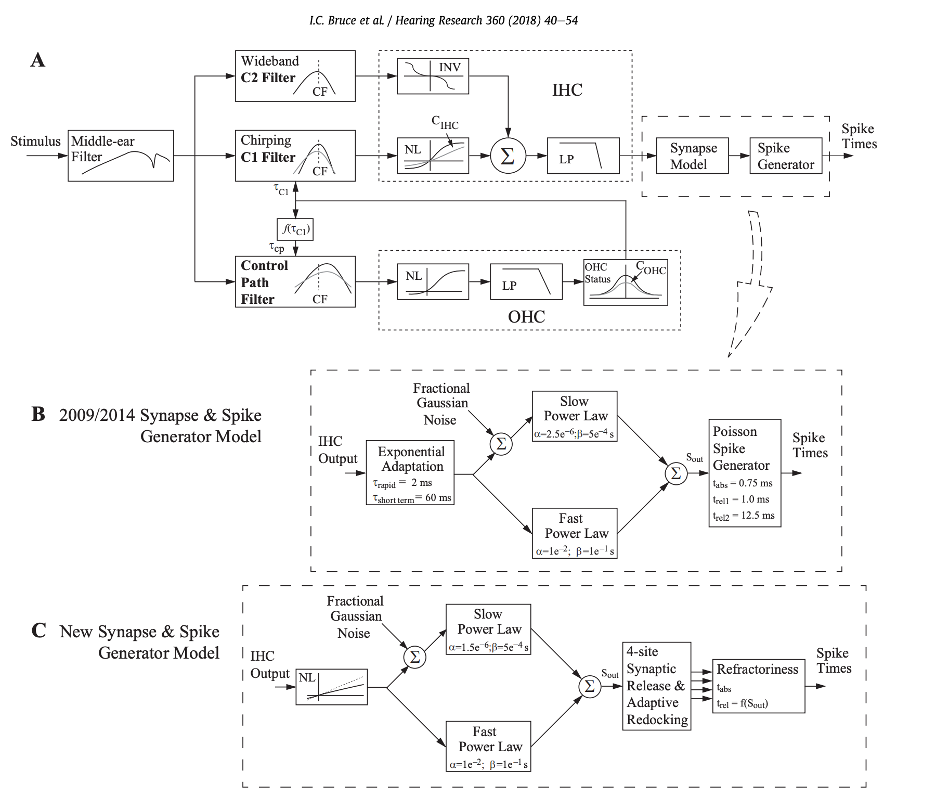
\includegraphics[width=\textwidth]{BruceModel}
	\caption[Schematic for \cite{bruce2018phenomenological} auditory periphery model]{Mammalian auditory periphery model used in the NSIM and STMI predictors of speech intelligibility \citep{bruce2018phenomenological}  \textbf{Ask Ian about premission}.}
	\label{fig:bruce_model}
\end{figure}

ANF spike patterns are often visualized via a neurogram which is a 2D representation of spike density as a function of CF and time (e.g., Figure \ref{fig:nsim_stmi}). Similar to a spectrogram, a neurogram describes how energy is distributed in time and acoustic frequency from a neurological perspective. As such, it provides a visual representation of spectro-temporal modulation cues which are used by the brain to decode speech.


\cite{hines2010speech} presented two different types of neurograms: an average discharge neurogram (i.e., mean-rate or envelope neurogram, ENV) and a fine timing neurogram (i.e., spike timing or temporal fine structure neurogram, TFS). Both are smoothed in time by filtering the spike pattern with a 50\% overlap hamming window. The mean-rate neurogram uses a longer window in the order of several milliseconds, while the spike timing neurogram uses a window in the order of several microseconds. In general, mean-rate neural cues have been shown to correlate more to envelop acoustic cues, and spike timing neural cues have been correlated more to temporal fine structure acoustic cues. 

\cite{hines2010speech} proposed an objective speech intelligibility predictor that used image processing of neurograms to compare the neural representation of a degraded signal to a clean reference signal. The degraded neurogram represents the result of a degraded acoustic signal and/or hearing impairment, while the clean reference represents a clean acoustic signal and normal hearing. The comparison is done using the structural similarity index (SSIM) which measures image quality based on comparison three measured parameters: luminance (i.e., intensity), contrast (i.e., variance), and structure (i.e., cross-correlation), i.e.,

\begin{equation}
	S(r,d)=l(r,d)^\alpha \cdot c(r,d)^\beta \cdot s(r,d)^\gamma \label{eq:SSIM}
\end{equation}

\noindent
where $r$ is the reference image, $d$ is the degraded image, $l$ is luminance, $c$ is contrast, $s$ is structure, and $\alpha$, $\beta$ and $\gamma$ are weights.

\cite{hines2012speech} developed the neurogram similarity index measure (NSIM) which improved upon the SSIM, providing optimal weighting values, and separately defining the mean-rate NSIM (MR NSIM)and fine timing NSIM (FT NSIM) for the respective neurogram types. The NSIM also dropped the contrast parameter for simplicity, since it was shown to have very little correlation to subjective speech intelligibility.

\cite{zilany2007predictions} extended the model to better represent how the central auditory system analyzes the effective spectrogram generated by the cochlear analysis and extracts the spectro-temporal modulation cues that are used to decode speech. This process is modeled as a bank of modulation-sensitive filters (i.e., a modulation filter bank), each having a corresponding impulse response called a spectro-temporal response field (STRF). Each STRF is centred around a certain time/frequency and is sensitive to a specific spectral modulation frequency (scale, i.e., density, in cycles/oct) and a specific temporal modulation frequency (rate, i.e., velocity, in \unit{\hertz}). The result is a 4D complex-valued analysis generated by convolving the auditory spectrogram with the bank of STRFs. This analysis is performed on the test signal and the clean reference signal, and the two results are compared by a 4-dimensional distance metric, resulting in the so-called spectro-temporal modulation index (STMI).

\begin{equation}
	\mathrm{STMI}=\sqrt{1-\frac{||T-N||^2}{||T||^2}} \label{eq:STMI}
\end{equation}

\noindent
where $T$ is the template stimulus (i.e., corresponds to the clean reference), and $N$ is the test stimulus (i.e., corresponds to the degraded signal/representation).

\begin{figure}[H]
	\centering
	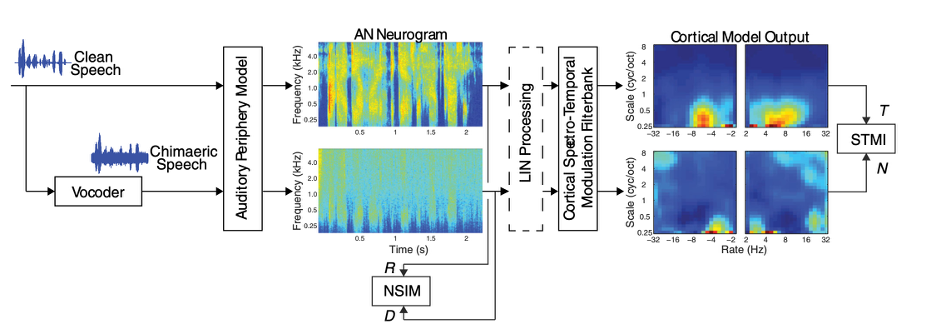
\includegraphics[width=\textwidth]{nsim_stmi}
	\caption[Schematic for generation of NSIM and STMI]{Schematic for generation of NSIM and STMI predictors of speech intelligibility. Note that the usage of Chimaeric speech as the test signal in this depiction is specific to the study being conducted by \citep{wirtzfeld2017predictions}. \textbf{Need permission}.}
	\label{fig:nsim_stmi}
\end{figure}

\cite{wirtzfeld2017predictions} performed a comparison of the STMI, mean-rate NSIM and spike-timing NSIM for estimation of subjective speech intelligibility, and found that a synthesis of STMI and spike-timing NSIM provided the most consistent results. 

While the auditory modeling described in this section is monaural, making is suboptimal for evaluating reverberation, an EC front-end could potentially be added to provide a simplistic model of binaural perceptual adaptations.


\subsection {Objective Predictors of Listening Effort}

As previously discussed, SI is only impacted by reverberation in severe conditions which are not typically experienced in every day life, but LE is impacted even in mild reverb. In other words as reverberation time decreases, SI increases and LE decreases, but SI eventually plateaus at 100\%, while LE continues to decrease. 

Objective predictors of SI such as STI continue to increase after subjective SI ratings plateau. These ceiling effects are accounted for by applying a nonlinear mapping from objective predictor of SI to subjective SI rating. However, it has been suggested that that the full range of these predictors can be used to predict LE due to the strong correlation between SI and LE over the range in which SI has not reached saturation \citep{schepker2016perceived}.

\subsection{Objective Predictors of Speech Quality}

As reviewed by \cite{torcoli2021objective}, several objective predictors of SQ have been proposed which aim to estimate subjective ratings such as MOS. Generally, this is done by extracting and analyzing quality features such as loudness, coloration, noisiness and distortion. One of the earliest and most common predictors is the perceptual evaluation of speech quality (PESQ) \citep{itu2003pesq} and its successor the perceptual objective listening quality assessment (POLQA) \citep{itu2011polqa}. Both of these predictors use a simplified perceptual model that emulates the time-frequency decomposition of the cochlea, and compare the extracted quality features of the degraded signal to a clean reference signal. More recently, \cite{hines2015visqol} proposed the virtual speech quality objective listener (VISQOL) which used an improved perceptual model. VISQOL was originally developed using the NSIM to compare the degraded and clean signals, but switched to using a spectrogram rather than a neurogram, which proved to be equally effective and much less complex. Compared to PESQ and POLQA, VISQOL has been shown to be less complex and equally effective at predicting subjective SQ \citep{hines2013robustness}. Similar to HASPI for SI, \cite{kates2022overview} proposed the hearing aid speech quality index (HASQI), which uses the same perceptual model as HASPI to predict SQ.

\section{Linear Prediction} \label{linear_prediction}

The concept of linear prediction (LP) was originally proposed by \cite{wiener1949extrapolation} in his seminal contributions on modeling discrete time signals as stochastic processes, and equivalently modeling filtering and prediction as a statistical problem. The first formal discussions of linear prediction in the context of speech signals were presented concurrently by \cite{saito1967theoretical} and \cite{atal1970adaptive}.

As described in Section \ref{dt_speech_model}, speech production can be roughly modeled as the excitation of time-varying all-pole filter with a source signal made up of a combination of ideal impulse trains, white noise and individual impulse spikes. Motivated by this source-filter/AR model of speech (Equation \ref{eq:AR_speech}), linear prediction was proposed as an efficient method for encoding speech by estimating and storing the poles of the effective all-pole vocal tract filter, and later using them to re-synthesize the original speech waveform. This is commonly used in speech codecs where the speech is broken into frames and the parameters of the source/filter model can be encoded at a lower bit rate than the raw sampled waveform.

The process of linear prediction can be viewed from three separate but related perspectives, namely as a method for predicting a signal, identifying/inverting a system (i.e., the speech production filter), and estimtaing/whitening the signal spectrum. These perspectives each present important insights. A detailed discussion of this linear prediction theory can be found in \cite{quatieri2002discrete}, but the important details have been summarized here.

\subsection{Signal Prediction Perspective} \label{lp_signal_perspective}

Posed as a prediction problem, the approximately AR model of speech motivates the prediction, $\hat{s}(n)$, of a speech signal, $s(n)$, from only its previous samples. i.e.,

\begin{equation}
	\hat{s}(n) = \sum_{k=1}^{p}\alpha_k s(n-k) \label{eq:lpc_prediction}
\end{equation}

\noindent
where $\{\alpha_k, k=1,\dots,p\}$ are referred to as the prediction coefficients. The corresponding prediction error (i.e., the prediction residual) is

\begin{equation}
	e(n)= s(n) - \hat{s}(n) =  s(n)  - \sum_{k=1}^{p}\alpha_k s(n-k) \label{eq:lpc_error}
\end{equation}


If the original speech signal is indeed an AR process, if the prediction order is sufficiently high, and if the poles of the effective speech production filter are correctly estimated (i.e., $\alpha_k=a_k, \; k=1,\dots,p$), Equation \ref{eq:lpc_prediction} exactly matches the equation for the AR model of speech (Equation \ref{eq:AR_speech}) and therefore the residual will be equal to the idealized excitation sequence, i.e., 

\begin{equation}
	e(n)\Bigm|_{\alpha_k=a_k, \; \forall k=1,\dots,p} = u(n) = 
	\begin{cases} 
		u_\mathrm{g}(n) & \text{during voiced speech} \\
		u_\mathrm{i}(n)  & \text{during unvoiced plosive speech} \\
		u_\mathrm{n}(n) & \text{during unvoiced fricative speech} \\
	\end{cases}
\end{equation}

In estimation of the coefficients of the all-pole model, the optimal prediction coefficients are found by minimizing prediction error in a mean squared error (MSE) sense. From a speech coding stand point, the MSE cost function is defined differentially when modeling voiced speech which is considered deterministic, and unvoiced fricative speech which is stochastic in nature. In the deterministic modeling case, MSE is defined as the total squared error over all time, i.e.,

\begin{eqnarray}
	J = \sum_{n=-\infty}^{\infty}e^2(n) = \sum_{n=-\infty}^{\infty} \left(s(n)  - \sum_{k=1}^{p}\alpha_k s(n-k)\right) ^2 \label{eq:lp_mse_deterministic}
\end{eqnarray}

Equivalently, in the stochastic modeling case, MSE is defined as the as the ensemble average (i.e., expectation) of the squared error process, i.e.,

\begin{eqnarray}
	J = E \left[ e^2(n) \right] = E\left[ \left(s(n)  - \sum_{k=1}^{p}\alpha_k s(n-k) \right) ^2\right]
\end{eqnarray}

\noindent
which can be exactly computed by time-averaging over all time (i.e., is exactly equivalent to Equation \ref{eq:lp_mse_deterministic}) provided $s(n)$ is an ergodic random process. Under this condition, the two formulations, and thus the resulting solutions, are identical.

The MSE metric is ideally computed/averaged over all time. However, in practice minimization is done for a short-term signal frame (i.e., prediction error interval) due to availability of a finite amount of data, and/or due to time-varying nature of speech which makes it only short-time stationary. In both the stochastic and deterministic cases, the MSE is estimated in this way, and thus their formulations/solutions are indeed identical in practice. The specific definition of short-term MSE in the vicinity of time $n$, denoted $J_n$, differs for the autocorrelation method and covariance method which will be discussed in the next section.

It turns out that the MSE cost function, $J$, forms a $(p+1)$-dimensional error surface which is a quadradic function of the prediction coefficients, with exactly one global minimum corresponding to the optimal set of coefficients (i.e., a quadratic bowl). Therefore the optimal solution, minimizing $J$, can be found by taking its partial derivative with respect to each prediction coefficient, and setting it equal to zero:

%Explain if needed:This can be shown by vector expansion, … , Leading to quadratic form, … Positive (semi?)definite implying a minimum

\begin{eqnarray}
	\{\alpha_k\} = \underset{\{\alpha_k\}}{\arg\min} \; J \\
	\frac{\partial J}{\partial \alpha_k}=0
\end{eqnarray}

From the orthogonality principle, the optimal solution will produce an error signal that is orthogonal to, and therefore uncorrelated with, the input signal except at a lag of zero (i.e., uncorrelated with a unit-delayed version of the speech signal). Since any autocorrelation in the residual also implies correlation between the residual and the input, the optimal prediction residual is also uncorrelated with itself except at a lag of zero, i.e.,

\begin{eqnarray}
	r_{es}(\tau) = E\left[e(n)s(n-\tau)\right] = 0 & \tau=0,\dots,p \label{eq:optimal_r_es} \\
	r_{ee}(\tau) = E\left[e(n)e(n-\tau)\right]=\delta(\tau)  & \tau=0,\dots,p  \label{eq:optimal_r_ee}
\end{eqnarray}

This makes intuitive sense because by optimally predicting and subtracting the part of the speech signal that can be predicted from its past samples, linear prediction exploits and removes temporal correlation from the signal. Since this is also the autocorrelation function of the idealized excitation sequence (impulse, pulse train or white noise), this reinforces that the optimal prediction residual will be the idealized excitation sequence and therefore the prediction coefficients will correspond to the AR parameters of the underlying process.

It is important to note that Equations  \ref{eq:optimal_r_es} and \ref{eq:optimal_r_ee} only hold for certain lags, which is dictated by the prediction order, $p$. This will be discussed more later.


\subsection{System Identification / Inverse Filtering Perspective} \label{lp_inverse_filtering_perspective}

In describing speech as the excitation of an all-pole filter with an idealized uncorrelated excitation sequence, we can also describe linear prediction as identification of the corresponding all-pole filter (i.e., system identification). 

In this context, the prediction coefficients form a $p$\textsuperscript{th} order FIR prediction filter $P(z)$, i.e.,

\begin{eqnarray}
	P(z) = \sum_{k=1}^{p}\alpha_k z^{-k} \\
	\hat{S}(z) = P(z)S(z)
\end{eqnarray}

\noindent
and a corresponding $p$\textsuperscript{th} order FIR prediction error filter, $A(z)$.

\begin{eqnarray}
	A(z) = 1 - P(z) = 1 - \sum_{k=1}^{p}\alpha_k z^{-k} \\
	E(z) = A(z)S(z) = S(z) - P(z)S(z) = S(z) - \hat{S}(z)
\end{eqnarray}

\noindent
where $S(z)$, $\hat{S}(z)$ and $E(z)$ are the Z-transforms of the speech signal, $s(n)$, $\hat{s}(n)$, and $e(n)$ respectively.

The inverse of the prediction error filter (i.e., the inverse filter in linear prediction theory), which is a $p$\textsuperscript{th} order all-pole filter, re-synthesizes the original speech signal when excited with the prediction residual, i.e.,

\begin{eqnarray}
	\frac{1}{A(z))} = \frac{1}{1 - P(z)} = \frac{1}{1 - \sum_{k=1}^{p}\alpha_k z^{-k}} \\
	S(z) = \frac{1}{A(z)} E(z)
\end{eqnarray}

The block diagrams corresponding to these three filters are shown in Figure \ref{fig:LP_Filters}.

\begin{figure}[H]
	\centering
	\begin{subfigure}[b]{0.49\textwidth}
		\centering
		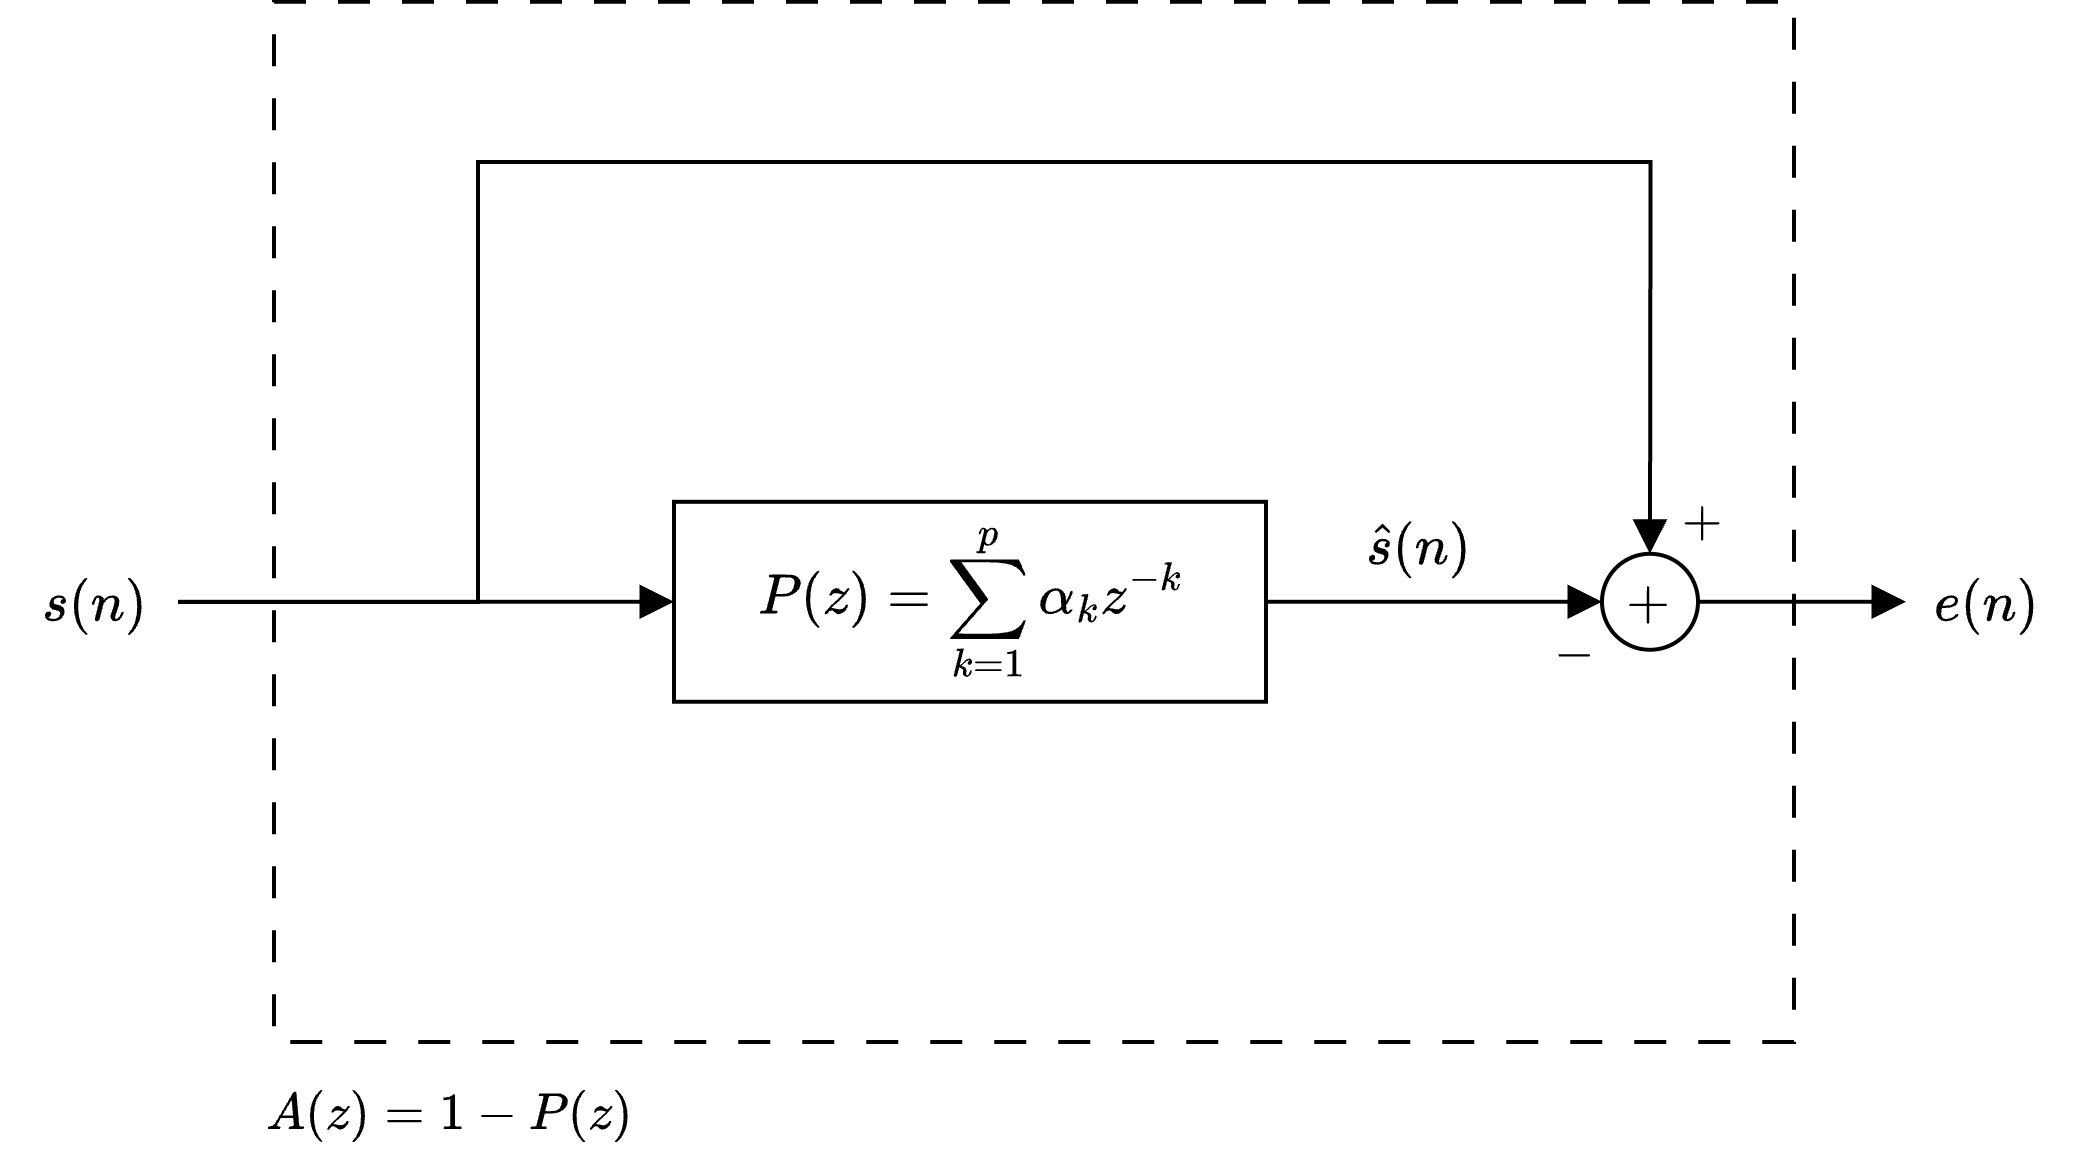
\includegraphics[width=\textwidth]{LP_PE_Filter}
		\subcaption{} \label{subfig:lp_pe_filter}
	\end{subfigure}
	\hfill
	\begin{subfigure}[b]{0.49\textwidth}
		\centering
		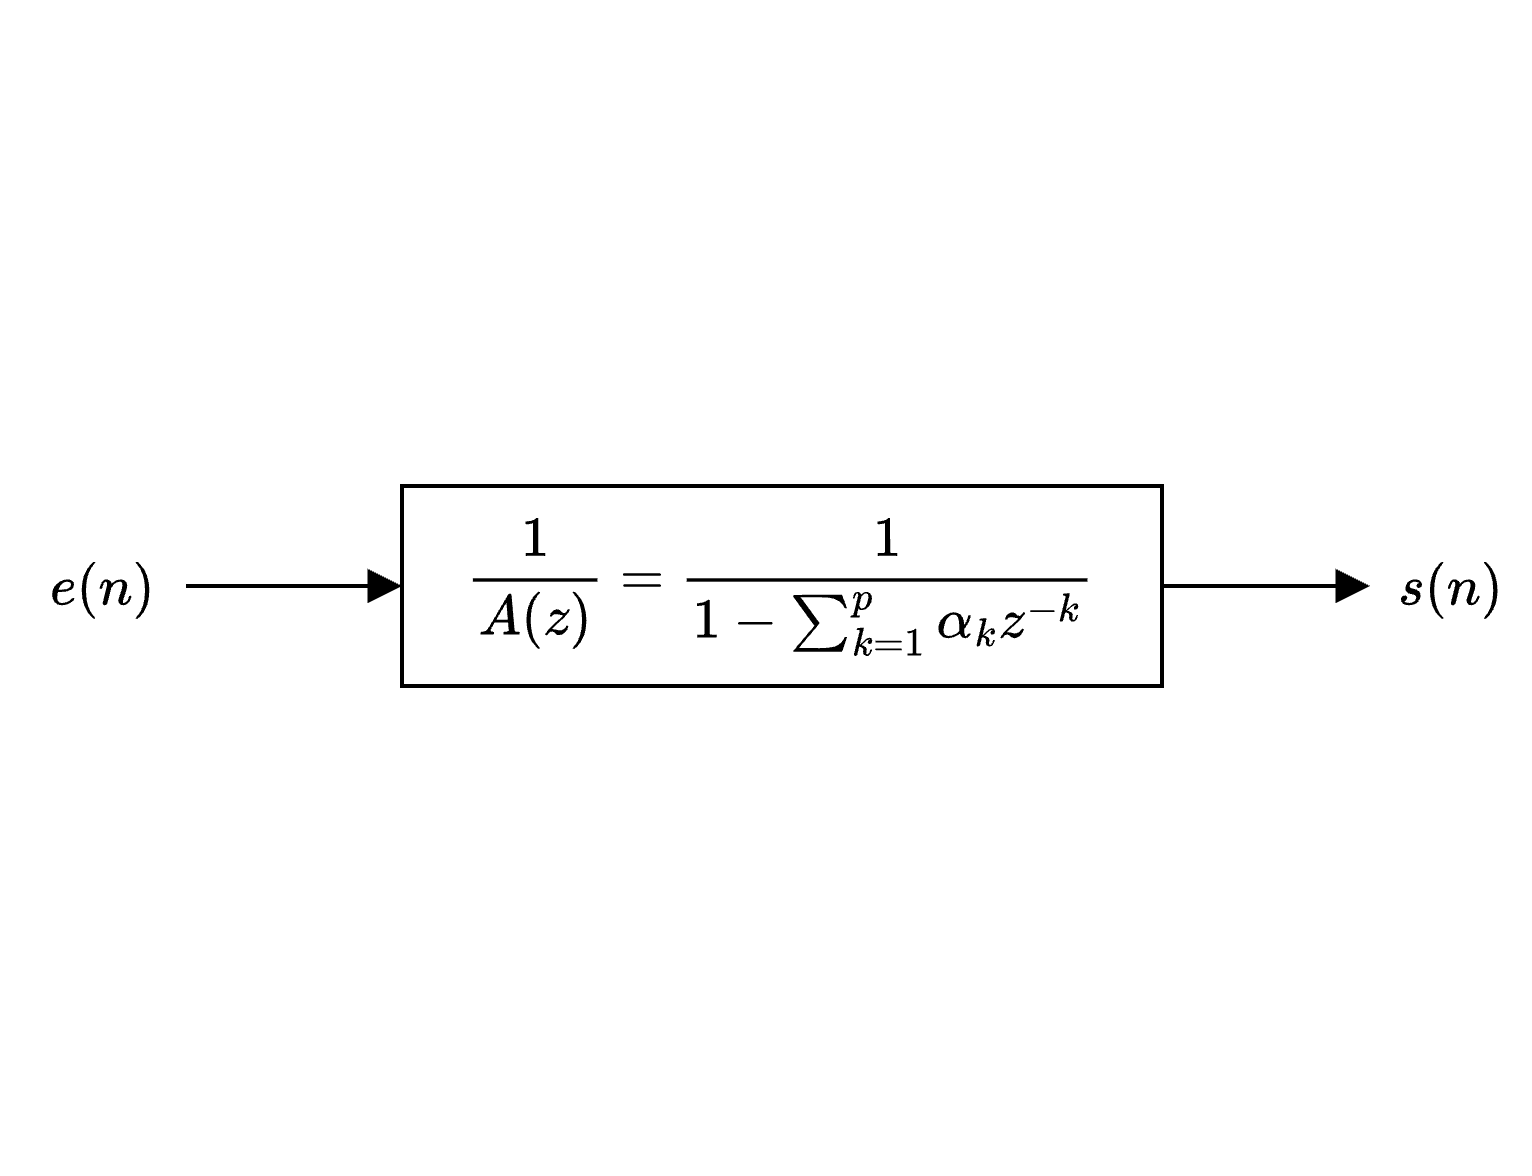
\includegraphics[width=\textwidth]{LP_Inverse_Filter}
		\subcaption{} \label{subfig:lp_inverse_filter}
	\end{subfigure}
	\caption[Block diagrams for filtering perspective of linear prediction]{Block diagram for LP prediction-error filter, $A(z)$ (a), and LP inverse filter,.$\frac{1}{A(z)}$ (b)}
	\label{fig:LP_Filters}
\end{figure}

If the $s(n)$ truly represents an the excitation of an all-pole system,  

\begin{eqnarray}
	H(z) = \frac{A}{1 - \sum_{k=1}^{p}a_k z^{-k}}
\end{eqnarray}

\noindent
where $A$ is a linear gain term to scale for signal amplitude, and if the prediction coefficients are correctly estimated (i.e., $\alpha_k=a_k, \; k=1,\dots,p$), the inverse filter will be identical to the actual all-pole system. Consequently, the prediction error filter will be the exact inverse of the all-pole system, i.e.,

\begin{eqnarray}
	\frac{1}{A(z)}\Bigm|_{\{\alpha_k\}=\{a_k\}}=H(z) \\
	A(z)=\frac{1}{H(z)}
\end{eqnarray}

If however the system has zeros, the linear prediction solution will be forced approximate these zeros with a finite number of poles in the inverse filter. As previously explained, an infinite number of poles are required to perfectly model a zero (Equation \ref{eq:zero_approx}), so the inverse filter will always be approximate when the true system has zeros.

When the all-pole inverse filter, $1/A(z)$,  is used for re-synthesis of the speech signal, careful attention must be given to ensure that it is stable (i.e., all poles must be inside the unit circle). This implies that the prediction error filter, generated by the optimization solution, must have all zeros inside the unit circle (i.e., minimum-phase). If the real system is truly a physical all-pole system, it will be inherently causal and stable, and therefore the optimization process will be able to achieve perfect prediction with a minimum phase prediction error filter. However, if the system has zeros, the all-pole model will be approximate, and in some cases it may be optimal to incorporate some maximum-phase zeros into the prediction error filter. Additionally, if the underlying process has acausal maximum-phase poles (e.g., the left-sided glottal pulse shape in speech production, Equation \ref{eq:glottal_pulse_z}), the optimal prediction error filter would include zeros at these locations, even though the inverse filter would be unstable.

To handle the issue of inverse filter stability, two different formulations of the optimization problem have been developed: the autocorrelation method and the covariance method. These two methods differ in their definition of the short-term MSE cost function, $J_n(n)$, which is to be minimized. 


%\textbf{TODO: Replace derivations uniquely in autocorrelation and covariance methods with simply subbing in different estimators of autocorrelation, and correlate them to the way error is defined, and subbing into expectation-based normal equations previously derived from a stochastic stand-point}

\subsubsection{Autocorrelation Method} \label{lp_autocor}

In the autocorrelation method, the speech signal is windowed to the prediction error interval $n \in [n, n+N_w-1]$ and the MSE is computed using error samples over all time, i.e.,

\begin{eqnarray}
	s_n(m) = s(m+n)w(m) \\
	e_n(m) = s_n(m) - \hat{s}_n(m) = s_n(m) - \sum_{k=1}^{p} \alpha_k s(m-k) \\
	J_n = \sum_{m=-\infty}^{\infty}e_n^2(m) = \sum_{m=0}^{N_w+p-1}e_n^2(m) \label{eq:autocorr_tse}
\end{eqnarray}

\noindent
where the subscript $n$ implies ``in the vicinity of time n", and $w(n)$ is the length-$N_w$ window function, which is non-zero only in the range $n \in [0, N_w-1]$. The window function could be rectangular, or some other non-uniform window (e.g., Hamming). Note that the change in summation bounds in Equation \ref{eq:autocorr_tse} is a result of the limited range of of non-zero elements in $e_n(n)$ due to the windowing of $s(n)$.

Minimization of $J_n$ with respect to the prediction cofficients (i.e., setting $\partial J_n  /\partial \alpha_k=0$) results in the so-called Yule-Walker equations. 

\begin{equation}
	\sum_{k=1}^{p} \alpha_k r_n(i-k) = r_n(i), \;\; i=1,\dots,p
\end{equation}

\noindent
where $r_n(\tau) = \sum_{m=0}^{N_w-1-\tau}s_n(m)s_n(m-\tau)$ is the short-term autocorrelation function of $s(n)$. This is simply the least-squares normal equations applied to linear prediction. The short-term autocorrelation function, which is a function of only time-lag as opposed to absolute time, appears due to the infinite summation over the error signal, and implies an inherit assumption of stationary speech. This implies that the signal is inheritly assumed to be a realization of a wide-sense stationary (WSS) ergodic stochastic process. In speech coding, where the goal is to model and encode the time-varying speech production system, the duration of analysis window (i.e., $N_w$) is selected short enough that speech mayb be considered approximately stationary, typically 20-30 \unit{\milli\sec}. However, when linear prediction is applied to system identification problems where the system is slower time-varying, a larger analysis window may be selected, in which case the statistics of speech are smoothed out and may be considered long-term stationary \citep{gazor2003speech}.

The Yule-Walker equations can be restated in matrix form as

\begin{eqnarray}
	\boldsymbol{R}_n \boldsymbol{\alpha} = \boldsymbol{r}_n \\
   	\begin{bmatrix} 
	   	r_n(0)    & r_n(1)      & r_n(2)     & \dots     & r_n(p-1)  \\
	   	r_n(1)     & r_n(0)      & r_n(1)     & \dots     & r_n(p-2)  \\
	   	r_n(2)     & r_n(1)      & r_n(0)     & \dots     & r_n(p-3)  \\
	   	\vdots     & \vdots      & \vdots     & \ddots  & \vdots  \\
	   	r_n(p-1)  & r_n(p-2)  & r_n(p-3) & \dots    & r_n(0)  \\
	\end{bmatrix} 
	\begin{bmatrix}
		\alpha_1 \\
		\alpha_2 \\
		\alpha_3 \\
		\vdots    \\
		\alpha_p \\
	\end{bmatrix}
	=
	\begin{bmatrix}
		r_n(1)  \\
		r_n(2) \\
		r_n(3) \\
		\vdots    \\
		r_n(p) \\
\end{bmatrix}
\end{eqnarray}

\noindent
which can be solved by matrix inversion

\begin{equation}
	 \boldsymbol{\alpha} = \boldsymbol{R}_n^{-1} \boldsymbol{r}_n
	 %\boldsymbol{R}_n^+ \boldsymbol{r}_n  = (\boldsymbol{R}_n^T \boldsymbol{R}_n)^{-1} \boldsymbol{R}_n^T  \boldsymbol{r}_n 
\end{equation}

The Toeplitz symmetric nature of the autocorrelation matrix, resulting from the underlying WSS assumption, additionally enables usage of the recursive Levinson-Durbin algorithm \citep{durbin1960fitting}. This algorithm is highly efficient compared to other methods of solving systems of linear equations, but is known to be prone to numerical instability due to its inherit recursion when the autocorrelation matrix is ill-conditioned.

It has been shown that due to the Toeplitz symmetric nature of the autocorrelation matrix $\boldsymbol{R}_n$, the autocorrelation method produces a minimum-phase prediction error filter. Therefore the resulting inverse filter used for speech re-synthesis is a stable all-pole filter. It has also been shown that the autocorrelation function of the inverse filter produced by the autocorrelation method is identical to the autocorrelation function of the signal being predicted, up to a lag of $p$, i.e.,

% It has also been shown that the autocorrelation method ($p$\textsuperscript{th} order LPC) produces a filter (i.e., the inverse filter) for which the first $p+1$ values of the autocorrelation function of the system impulse response, $h(n)=Z^{-1}\{H(z)\}$, is identical to the first $p+1$ autocorrelation values of the signal, i.e.,

%It has also been shown that the IR of the inverse filter produced by the autocorrelation method (i.e., $h(n)=Z^{-1}\{H(z)\}$) has an IR for which the first $p+1$ values of the autocorrelation function of the system impulse response is identical to the first $p+1$ autocorrelation values of the signal, i.e.,

\begin{eqnarray}
	r_{\hat{h}}(\tau) = r_s(\tau) \;\; \tau=0, \dots, p
\end{eqnarray}

\noindent
where $\hat{h}(n)=Z^{-1}\{\frac{1}{A(z)}\}$. Since the autocorrelation function completely defines the power spectral density (i.e., PSD is the fourier transform of the autocorrelation function), it can be concluded that the magnitude response of the inverse filter is identical to that of the true system up to a spectral resolution defined by the prediction order. Therefore, for large enough prediction orders, the inverse filter resulting from the autocorrelation method represents the equivalent minimum phase representation of the true system. That is, if the true system, $H(z)$ is non-minimum phase and we decompose it into its equivalent minimum phase and all-pass components,

\begin{eqnarray}
	H(z) = H_{\mathrm{min}}(z) H_{\mathrm{allpass}}(z) \\
	\| H_{\mathrm{min}}(z) \| = \| H(z) \|  \\
\end{eqnarray}

\noindent
then as $p \rightarrow \infty$, $\frac{1}{A(z)} \rightarrow H_{\mathrm{min}}(z)$, and

\begin{equation}
	H(z) A(z) = H_{\mathrm{allpass}}(z) 
\end{equation}

However the windowing of the speech signal prior to error calculation means that only part of the infinite-length system impulse response will be captured in the autocorrelation function. This can result in distortion of the estimated all-pole inverse filter, an effect that can be minimized but never avoided entirely by using a longer window. When attempting to model the vocal tract as an all-pole filter, the window must also be short enough that the signal is considered short-time stationary, otherwise the analyzed spectrum will be smoothed by the time-varying nature of speech. The window size thus represents a trade off between capturing short-time spectra and capturing the entirety of the IIR system impulse response. 

To summarize, the autocorrelation method can therefore be described as a biased solution, which may be sub-optimal in an MSE sense. The resulting prediction error filter is guaranteed to be minimum phase, and the resulting inverse filter is guaranteed to be a stable minimum-phase filter that matches the magntitude response of the true system up to a spectral resolution defined by the prediction order.


\subsubsection{Covariance Method} \label{lp_cov}

In the covariance method, the speech signal is not windowed, but the prediction error is computed using error samples only within the prediction error interval $n \in [n, n+N_w-1]$. This means that the error samples are computed using samples outside of the prediction error interval, and thus represent the true error signal over the entire interval, i.e.,

\begin{eqnarray}
	s_n(m) = s(m+n) \\
	e_n(m) = s_n(m) - \hat{s}_n(m) = s_n(m) - \sum_{k=1}^{p} \alpha_k s(m-k) \\
	J_n = \sum_{m=0}^{N_w-1} e_n^2(m) \label{eq:cov_tse}
\end{eqnarray}

 Minimization of short-term MSE, $J_n$, with respect to the prediction coefficients (i.e., setting $\partial J_n/\partial \alpha_k=0$) results in a different set of normal equations in terms of the short-term covariance function. 
 
 \begin{equation}
 	\sum_{k=1}^{p} \alpha_k \phi_n(i,k) = \phi_n(i,0)
 \end{equation}
 
 \noindent
 where $\phi_n(i,k) = \sum_{m=0}^{N_w-1} s_n(m-i) s_n(m-k)$ is the short-term covariance. It is important to note that by convention in signal processing theory, short-term covariance is not used to mean the short-term parallel of long-term covariance. While long-term covariance is formally defined as the autocorrelation function with its mean removed, short-term covariance is defined as the short-term parallel of non-stationary correlation. In other words short-term correlation is a function of lag and implies analysis of stationary processes, while short-term covariance is a function of two time instances and implies analysis of non-stationary processes.
 
 The covariance method normal equations can also be represented in matrix form.
 
 \begin{eqnarray}
 	\boldsymbol{\Phi}_n \boldsymbol{\alpha} = \boldsymbol{\phi}_n \\
 	\begin{bmatrix} 
 		\phi_n(1,1)   & \phi_n(1,2)   & \phi_n(1,3)     & \dots    & \phi_n(1,p)  \\
 		\phi_n(2,1)   & \phi_n(2,2)  & \phi_n(2,3)     & \dots     & \phi_n(2,p)  \\
 		\phi_n(3,1)   & \phi_n(3,2)  & \phi_n(3,3)     & \dots    & \phi_n(3,p)  \\
 		\vdots      & \vdots      & \vdots          & \ddots  & \vdots  \\
 		\phi_n(p,1)  & \phi_n(p,2)  & \phi_n(p,3)      & \dots    & \phi_n(p,p)  \\
 	\end{bmatrix} 
 	\begin{bmatrix}
 		\alpha_1 \\
 		\alpha_2 \\
 		\alpha_3 \\
 		\vdots    \\
 		\alpha_p \\
 	\end{bmatrix}
 	=
 	\begin{bmatrix}
 		\phi_n(1)  \\
 		\phi_n(2) \\
 		\phi_n(3) \\
 		\vdots    \\
 		\phi_n(p) \\
 	\end{bmatrix}
 \end{eqnarray}
 
 \noindent
which can be solved by matrix inversion
 
 \begin{equation}
 	\boldsymbol{\alpha} = \boldsymbol{\Phi}_n^{-1} \boldsymbol{\phi}_n
 	%\boldsymbol{\Phi}_n^+ \boldsymbol{\phi}_n  = (\boldsymbol{\Phi}_n^T \boldsymbol{\Phi}_n)^{-1} \boldsymbol{\Phi}_n^T  \boldsymbol{\phi}_n 
 \end{equation}
 
The covariance matrix is symmetric but not Toeplitz, therefore more correlation coefficients must be calculated compared to the autocorrelation method, and it cannot be solved efficiently with the Levinson-Durbin algorithm. However covariance matrices are usually positive definite allowing use of Cholesky decomposition \citep[][chapter 5]{reilly2025fundamentals}. Cholesky is less efficient than the Levinson-Durbin algorithm but is more numerically stable.

Unlike the autocorrelation method where windowing enforces an implicit stationary assumption and derives a minimum-phase prediction error filter, the covariance method represents an unconstrained/unbiased optimization problem. As such the covariance method tends to perform better than the autocorrelation method when the system/process is known to be non-stationary, since the time-varying statistics are captured in the covariance matrix and used in the optimization. Being unconstrained, the covariance method may derive a non-minimum phase prediction error filter in cases where such a filter achieves a lower prediction error (e.g., in some cases when the underlying process includes zeros and/or acausal maximum phase poles). The covariance method is only guaranteed to come up with a minimum-phase prediction error filter if the underlying process is indeed minimum-phase all-pole. It is important to note however, that the prediction error filter is only required to be minimum-phase if the inverse filter is intended to be used for speech re-synthesis (e.g., speech codecs). In some cases, only the prediction error filter is used (e.g., equalizer/whitening filter design), in which case the non-minimum phase solution may be prefereable.

Additionally, while the windowing in the autocorrelation method means that the modeling of the true all-pole system is always approximate (except as the window size approaches infinity), the covariance method can perfectly estimate the coefficients of an all-pole system with only a finite number of data points.

To summarize, the covariance method represents an unbiased solution for the optimal prediction error filter (in a MSE sense) which may outperform the minimum-phase solution produced by the autocorrelation method if the underlying system/process is non-stationary, not all-pole, or has non-minimum phase acausal poles. However, the covariance method is more computationally complex and does not guarantee that the inverse filter used for speech re-synthesis will be stable.

\subsection{Spectral Estimation / Spectral Whitening Perspective}

The process of linear prediction can also be viewed as an estimation of the speech spectrum or the speech spectrum envelope. In the previous section, speech was modeled as the excitation of an all-pole filter with an uncorrelated input sequence. Under these conditions, it was explained that the autocorrelation method produces an inverse filter with an impulse response that has an autocorrelation function matching that of the signal, up to $p+1$ lags. It was explained that the resulting inverse filter exactly matches the magnitude response of the all-pole speech production filter, up to a spectral resolution defined by the prediction order. Identically, if the signal being analyzed is a realization of an AR process (i.e., the output of the system previously described), the autocorrelation method will generate an inverse filter with a magnitude response that exactly matches the signal  spectrum up to a spectral resolution defined by the prediction order

Similarly, the prediction error filter represents the inverse of the signal spectrum and therefore flattens it. This explanation aligns with the prediction perspective previously outlined, since the autocorrelation of the optimal solution was found to be an impulse, which corresponds to a flat PSD. It also aligns with the previous inverse filtering perspective where the prediction error filter inverts and therefore equalizes (i.e., whitens) the all-pole speech production filter. For this reason the prediction error filter is commonly referred to as a whitening filter. 

In speech spectrum analysis, it may be desirable to use a lower prediction order which underfits the spectrum, so as to only model the vocal tract resonances and spectral tilt (i.e., model the speech spectrum envelope). If the spectral resolution is increased too much, the inverse filter will begin to model not only the spectral envelope, but also the harmonics of glottal pulsing during voiced speech. This is undesirable in many speech codecs where the goal is to generate a model of the vocal tract and use it to resynthesize the speech signal using synthetically generated impulse trains.

%\section{Summary}



